\documentclass[a4paper]{article}

\setlength{\parindent}{0pt}
\setlength{\parskip}{1em}

\pagestyle{headings}

\usepackage{amssymb}
\usepackage{amsmath}
\usepackage{amsthm}
\usepackage{mathtools}
\usepackage{graphicx}
\usepackage{hyperref}
\usepackage{color}
\usepackage{microtype}
\usepackage{tikz}
\usepackage{pgfplots}
\usepackage{pgfplotstable}

\newcommand{\N}{\mathbb{N}}
\newcommand{\Q}{\mathbb{Q}}
\newcommand{\Z}{\mathbb{Z}}
\newcommand{\R}{\mathbb{R}}
\newcommand{\C}{\mathbb{C}}
\newcommand{\D}{\mathcal{D}}
\renewcommand{\S}{\mathcal{S}}
\renewcommand{\P}{\mathbb{P}}
\newcommand{\F}{\mathbb{F}}
\newcommand{\E}{\mathbb{E}}
\newcommand{\bra}{\langle}
\newcommand{\ket}{\rangle}


\graphicspath{{Image/}}

\hypersetup{
    colorlinks=true,
    linktoc=all,
    linkcolor=blue
}

\theoremstyle{definition}
\newtheorem*{axiom}{Axiom}
\newtheorem*{claim}{Claim}
\newtheorem*{conv}{Convention}
\newtheorem*{coro}{Corollary}
\newtheorem*{defi}{Definition}
\newtheorem*{eg}{Example}
\newtheorem*{lemma}{Lemma}
\newtheorem*{notation}{Notation}
\newtheorem*{prob}{Problem}
\newtheorem*{post}{Postulate}
\newtheorem*{prop}{Proposition}
\newtheorem*{rem}{Remark}
\newtheorem*{thm}{Theorem}

\DeclareMathOperator{\vdiv}{div}
\DeclareMathOperator{\grad}{grad}
\DeclareMathOperator{\curl}{curl}
\DeclareMathOperator{\Ann}{Ann}
\DeclareMathOperator{\Fit}{Fit}
\DeclareMathOperator{\Diag}{Diag}
\DeclareMathOperator{\tr}{tr}
\DeclareMathOperator{\im}{im}
\DeclareMathOperator{\Mat}{Mat}
\DeclareMathOperator{\Log}{Log}
\DeclareMathOperator{\Isom}{Isom}
\DeclareMathOperator{\Mesh}{Mesh}
\DeclareMathOperator{\Sym}{Sym}
\DeclareMathOperator{\Aut}{Aut}
\DeclareMathOperator{\cosech}{cosech}
\DeclareMathOperator{\Card}{Card}
\DeclareMathOperator{\Gal}{Gal}


\begin{document}

\title{Vector Calculus}
\date{Lent 2016}

\maketitle

\newpage

\tableofcontents

\newpage

\section{Differential operators}
\subsection{grad, div, curl}

View $\nabla f=\left(\frac{\partial f}{\partial x},\frac{\partial f}{\partial y},\frac{\partial f}{\partial z}\right)$ as obtained from $f$ by applying the vector operator:\\
$\nabla = \left(\frac{\partial}{\partial x},\frac{\partial}{\partial y},\frac{\partial}{\partial z}\right) = \mathbf{e_{i}} \frac{\partial}{\partial x_{i}}$,
where $\mathbf{e_{i}}$ is an orthonormal, right-handed system,
$\mathbf{e_{i}}\cdot \mathbf{e_{j}} = \delta_{ij}$, $\mathbf{e_{i}}\times \mathbf{e_{j}} = \epsilon_{ijk} \mathbf{e_{k}}$.\\
Call it \emph{grad}, write $\nabla f = \grad f$.\\
Now define
\begin{equation*}
\begin{aligned}
\nabla \cdot \mathbf{F} &= \left(\mathbf{e_{i}}\frac{\partial}{\partial x_{i}}\right)\left(F_{j} \mathbf{e_{j}}\right)\\
&= \frac{\partial F_{i}}{\partial x_{i}}\\
&= \frac{\partial F_1}{\partial x} + \frac{\partial F_2}{\partial y} + \frac{\partial F_3}{\partial z}.
\end{aligned}
\end{equation*}
Also written as $\vdiv \mathbf{F}$, called \emph{divergence} of $\mathbf{F}$.\\
And\\
\begin{equation*}
\begin{aligned}
\nabla \times\mathbf{F} &= \left(\mathbf{e_{i}}\frac{\partial}{\partial x_{i}}\right)\times\left(F_j\mathbf{e_{j}}\right)\\
&= \epsilon_{ijk} \frac{\partial F_j}{\partial x_i}\mathbf{e_k}.
\end{aligned}
\end{equation*}
Also written as $\curl \mathbf{F}$.\\
write $\left(\partial_1,\partial_2,\partial_3\right)=\left(\frac{\partial}{\partial x},\frac{\partial}{\partial y},\frac{\partial}{\partial z}\right)$, then
\begin{equation*}
\begin{aligned}
\curl \mathbf{F} &=
\begin{vmatrix}
\mathbf{e_1}& \mathbf{e_2}& \mathbf{e_3}\\
\partial_1& \partial_2& \partial_3\\
F_1& F_2& F_3
\end{vmatrix}\\
&=\left(\partial_2 F_3-\partial_3 F_2,\partial_3 F_1-\partial_1 F_3,\partial_1 F_2,\partial_2 F_1\right).
\end{aligned}
\end{equation*}
Note: with $\nabla$, order is important. e.g.:\\
$\mathbf{F}\cdot\nabla=F_i \frac{\partial}{\partial x_i}$ is a scalar operator;\\
$\nabla\cdot\mathbf{F}=\frac{\partial F_i}{\partial x_i}$ is a scalar function.\\
$\grad,\vdiv,\curl$ are all linear operators.\\
Leibniz properties hold for all of them:\\
\begin{equation*}
\begin{aligned}
\nabla\left(fg\right)=\left(\nabla f\right)g+f\left(\nabla g\right);\\
\nabla\cdot\left(f\mathbf{F}\right)=\left(\nabla f\right)\cdot\mathbf{F}+f\vdiv \mathbf{F};\\
\curl\left(f\mathbf{F}\right)=\left(\nabla f\right)\times\mathbf{F}+f\curl\mathbf{F}.
\end{aligned}
\end{equation*}
Also many more (can be proven by index notation):\\
\begin{equation*}
\begin{aligned}
\nabla\cdot\left(\mathbf{F\times\mathbf{G}}\right)&=\left(\nabla\times\mathbf{F}\right)\cdot\mathbf{G}-\mathbf{F}\cdot\left(\nabla\times\mathbf{G}\right);\\
\nabla\times\left(\mathbf{F}\times\mathbf{G}\right)&=\mathbf{F}\left(\nabla\cdot\mathbf{G}\right)-\mathbf{G}\left(\nabla\cdot\mathbf{F}\right)+\mathbf{G}\left(\nabla\cdot\mathbf{F}\right)-\mathbf{F}\left(\nabla\cdot\mathbf{G}\right);\\
\nabla\left(\mathbf{F}\cdot\mathbf{G}\right) &= \mathbf{F}\times\left(\nabla\times\mathbf{G}\right)+\mathbf{G}\times\left(\nabla\times\mathbf{F}\right)+\left(\mathbf{F}\cdot\nabla\right)\mathbf{G}+\left(\mathbf{G}\cdot\nabla\right)\mathbf{F}.
\end{aligned}
\end{equation*}

\begin{eg}
Recall $\left(\mathbf{a}\times\mathbf{b}\right)_k=\epsilon_{ijk}a_i b_j$.\\
So:\\
\begin{equation*}
\begin{aligned}
\nabla\cdot\left(\mathbf{F}\times\mathbf{G}\right)&=\frac{\partial}{\partial x_i}\left(\mathbf{F}\times\mathbf{G}\right)_i\\
&=\frac{\partial}{\partial x_i}\left(\epsilon_{ijk}F_j G_k\right)\\
&=\epsilon_{ijk}\frac{\partial F_j}{\partial x_i} G_k + \epsilon_{ijk} F_j \frac{\partial G_k}{\partial x_i}\\
&=\left(\nabla\times\mathbf{F}\right)_k\cdot\mathbf{G}-F_j \epsilon_{ikj}\frac{\partial G_k}{\partial x_i}\\
&=\left(\nabla\times\mathbf{F}\right)\cdot\mathbf{G}-\mathbf{F}\cdot\left(\nabla\times\mathbf{G}\right).
\end{aligned}
\end{equation*}
\end{eg}

\begin{eg}
Let $\mathbf{r}=\left(x,y,z\right)$. $r=\sqrt{x^2+y^2+z^2}$.\\
Calculate $\vdiv \left(r^\alpha\mathbf{r}\right) = \left(\nabla\left(r^\alpha\right)\right)\cdot\mathbf{r}+r^\alpha\left(\nabla\cdot\mathbf{r}\right)$.\\
But
\begin{equation*}
\begin{aligned}
\nabla r^\alpha &= \alpha r^{\alpha-1} \nabla r\\
&=\alpha r^{\alpha-1}\left(\frac{1}{r}\right)\left(x,y,z\right)\\
&=\alpha r^{\alpha-2}\mathbf{r},\\
\nabla\cdot\mathbf{r} = \frac{\partial x}{\partial x} + \frac{\partial y}{\partial y} + \frac{\partial z}{\partial z} = 3.
\end{aligned}
\end{equation*}

So
\begin{equation*}
\begin{aligned}
\vdiv\left(r^\alpha \mathbf{r}\right)&=\left(\alpha r^{\alpha-2}\mathbf{r}\right)\cdot\mathbf{r}+3r^\alpha\\
&=\alpha r^\alpha + 3r^\alpha;\\
\curl\left(r^\alpha\mathbf{r}\right)&=\nabla\left(r^\alpha\right)\times\mathbf{r}+r^\alpha\left(\nabla\times\mathbf{r}\right)\\
&=\mathbf{0}+\mathbf{0}\\
&=\mathbf{0}.
\end{aligned}
\end{equation*}
\end{eg}

\subsection{Second order derivatives}
We have\\
$\nabla\times\left(\nabla f\right)=\mathbf{0}$ for any $f$ -- "$\curl\grad=0$";\\
$\nabla\cdot\left(\nabla\times\mathbf{A}\right)=0$ for any $\mathbf{A}$ -- "$\vdiv\curl=0$".\\
Converse results also hold for suitable regions $D \subset \R^n$.\\
1) If $\mathbf{F}$ is defined on all $\R^3$ ( or any simply connected region $D$), then $\nabla\times\mathbf{F}=0 \implies \mathbf{F}=\nabla\varphi$ for some $\varphi$.\\
(freedom: $\varphi \to \varphi +$ constants also works)\\
2) If $\mathbf{F}$ is defined on all $\R^3$ ( or any $D \subset \R^3$ such that any sphere on $D$ can be contracted continuously to a point in $D$), then $\vdiv \mathbf{F}=0 \implies \mathbf{F}=\nabla\times\mathbf{A}$.\\
(freedom: $\mathbf{A}\to\mathbf{A}+\nabla\varphi$, called the gauge freedom of $\mathbf{A}$)\\

\begin{defi}
A vector field is called:\\
1)\emph{irrotational} if $\nabla\times\mathbf{F}=0$;\\
2)\emph{conservative} if $\mathbf{F}=\nabla\varphi$ for some $\varphi$;\\
3)\emph{solenoidal} if $\nabla\cdot\mathbf{F}=0$.
\end{defi}

\textbf{Laplacian operator}, $\nabla^2=\nabla\cdot\nabla=\frac{\partial^2}{\partial x^2}+\frac{\partial^2}{\partial y^2}+\frac{\partial^2}{\partial z^2}$.

For scalar fields $f$,

\begin{equation*}
\nabla^2f=\nabla\cdot\left(\nabla f\right)=\vdiv\left(\grad f\right).
\end{equation*}

For vector fields $\mathbf{F}=\left(F_{1},F_{2},F_{3}\right)$,
\begin{equation*}
\begin{aligned}
\nabla^2\mathbf{F}&=\nabla\left(\nabla\cdot\mathbf{F}\right)-\nabla\times\left(\nabla\times\mathbf{F}\right)\\
&=\grad\left(\vdiv\mathbf{F}\right)-\curl\left(\curl\mathbf{F}\right).
\end{aligned}
\end{equation*}

\begin{eg} (irrotational and conservative fields).\\
	Consider $\mathbf{F}=\left(-\frac{y}{x^2+y^2},\frac{x}{x^2+y^2},0\right)$:
	Check that $\nabla\times\mathbf{F}=0$.\\
	Consider $f\left(x,y,z\right)=\arctan \frac{y}{x}$:
	$\frac{\partial f}{\partial x}=-\frac{y}{x^2+y^2},\frac{\partial f}{\partial x}=-\frac{x}{x^2+y^2}$.\\
	It looks like $\mathbf{F}=\nabla f$, but $\arctan \frac{y}{x}$ is not continuous on whole of $\R^3-$(z axis)$=D$.\\
	Note that $\arctan \frac{y}{x}=$polar angle $\varphi$ in x-y plane.\\
	At $A$: $\varphi = 0$.\\
	Insist that $\varphi$ varies continuously along the curve. Then must have $\varphi=2\pi$ at $B$. But $B=A$.\\
	Now $\mathbf{F}$ is defined on $D$, so $\mathbf{F}\neq\nabla f$ on all $D$ with $f$ smooth.\\
	So $\mathbf{F}$ is not conservative on all $D$($D$ is not simply connected).\\
	Remove offending part, e.g. z-x plane for $x\geq 0$.\\
	$D'=\R-\left\{(\text{z axis})\cup(\text{z-x plane},x\geq 0)\right\}$.\\
	Then on $D'$, $\mathbf{F}=\nabla f$ everywhere and $f$ is smooth, i.e. $\mathbf{F}$ is conservative on $D'$. Also $D'$ is simply connected.
	
\end{eg}

\newpage

\section{Integral Theorems}
\subsection{Green's Theorem}
\begin{thm} (Green's)\\
	For smooth functions $P\left(x,y\right)\text{ and }Q\left(x,y\right)$,\\
	\begin{equation*}
	\int_{A} \left(\frac{\partial Q}{\partial x}-\frac{\partial P}{\partial y}\right) dA = \int_{C} \left(Pdx+Qdy\right).
	\end{equation*}\\
	Where $A$ is a simple bounded region in x-y plane, i.e. with boundary $\partial A=C$ a piecewise smooth, non-self intersecting closed curve, and it is traversed \emph{anticlockwise}.\\
	Equivalently, $A$ is on the left hand side of direction of traverse.
\end{thm}

\begin{eg}
	Let $P=x^2 y, Q=xy^2$.\\
	Green's theorem says:\\
	\begin{equation*}
	\int_{A} \left(y^2-x^2\right)dA = \int_{C}\left(x^2 ydx+xy^2 dy\right)
	\end{equation*}
	for any simple $A$, and $C$ is the boundary of $A$ traversed anticlockwise.\\
\end{eg}

\begin{rem}
Green's theorem holds also for non-simple regions $A\subseteq \R^2$, with holes -- having $C=\partial A$ being a number of disconnected components.\\
Orientations of $\partial A$ must always be chosen to have $A$ on the left-hand-side for direction of traverse.\\
\end{rem}

\subsection{Stoke's Theorem}
\begin{thm}(Stoke's)\\
	For a smooth vector field $\mathbf{F}\left(\mathbf{r}\right)$,\\
	\begin{equation*}
	\int_{S} \left(\nabla\times\mathbf{F}\right)\cdot d\mathbf{S} = \int_{C}\mathbf{F}\cdot d\mathbf{r}.
	\end{equation*}
	where $S$ is a smooth bounded surface with boundary $\partial S=C$,piecewise smooth, non-self intersecting closed curve(or a union of such, \underline{and} $S$ and $C$ have \emph{compatible orientations}, i.e. if $mathbf{n}$ is normal to $S$ and $\mathbf{t}$ is unit tangent to $C$(so that $d \mathbf{S}=\mathbf{n}dS, d \mathbf{r}=\mathbf{t}dS, S=\text{arclength}$), then "if stand on boundary with head up in direction of $\mathbf{n}$ and face direction $\mathbf{t}$, then $S$ is on the left hand side." $\mathbf{t}\times\mathbf{n}$(which is tangent to $S$ too) points \underline{out} from $S$ along $C$.
\end{thm}

\begin{eg}
Consider $S=$Section of sphere of radius $a$ for $0\leq \theta \leq \alpha$.\\
Spherical polar coordinates ($r=a,\theta,\varphi$).\\
Orient $S$ with outward pointing normal $\mathbf{n}=\mathbf{e_{r}}$.\\
Then compatible orientation for $C$ is anticlockwise looking down from north pole, i.e. in direction of \emph{increasing} $\varphi$ when $C$ is parameterised by $\varphi$.\\
$S$ is $\theta : 0\to \alpha$, $\varphi:0\to 2\pi$ in $\left(\theta,\varphi\right)$ parameters.\\
$\mathbf{r}\left(\theta,\varphi\right) = \left(a\sin\theta\cos\varphi,a\sin\theta\sin\varphi,a\cos\theta\right)$.\\
So find the partial derivatives of $\mathbf{r}$ with respect to $\theta$ and $\varphi$, and get
$|\frac{\partial \mathbf{r}}{\partial\theta}\times\frac{\partial\mathbf{r}}{\partial \varphi}|=a^2 \sin\theta$.\\
so $d\mathbf{S}=a^2 \sin\theta \mathbf{e_{r}}d\theta d\varphi$.\\
For $C$: $r=a$ and $\theta=\alpha$:\\
$\mathbf{r}\left(\varphi\right)=\left(a\sin\alpha\cos\varphi,a\sin\alpha\sin\varphi,a\cos\alpha\right)$.\\
$d\mathbf{r}=\frac{d\mathbf{r}}{d\varphi}d\varphi=a\sin\alpha\left(-\sin\varphi,\cos\varphi,0\right)d\varphi$.\\
Stokes says:
\begin{equation*}
\int_{S} \left(\nabla\times\mathbf{F}\right)\cdot \mathbf{dS} = \int_{C}\mathbf{F}\cdot\mathbf{dr}.
\end{equation*}
So e.g. take $\mathbf{F}=\left(0,xz,0\right)$,\\
have $\nabla\times\mathbf{F}=\left(-x,0,z\right)$.\\
So
\begin{equation*}
\begin{aligned}
\left(\nabla\times\mathbf{F}\right)\cdot\mathbf{dS}&=\left(-x,0,z\right)\cdot\mathbf{e_{r}}r d\theta d\varphi\\
&=\left(-a\sin\theta\cos\varphi,0,a\cos\theta\right)\cdot\left(\sin\theta\cos\varphi,\sin\theta\sin\varphi,\cos\theta a^2 \sin\theta d\theta d\varphi\right)\\
&=\left(-a^3 \sin^3 \theta \cos^2 \varphi + a^3 \sin\theta\cos^2 \theta\right) d\theta d\varphi\\
\end{aligned}
\end{equation*}
\begin{equation*}
\begin{aligned}
\mathbf{F}\cdot\mathbf{dr}&=\left(0,xz,0\right)\cdot\left(-sin\varphi,\cos\varphi,0\right)a\sin\alpha d\varphi\\
&=a^3 \sin^2 \alpha\cos\alpha\cos^2 \varphi d\varphi\\
\end{aligned}
\end{equation*}
So
\begin{equation*}
\begin{aligned}
\int_{S} \left(\nabla\times\mathbf{F}\right)\cdot\mathbf{dS}=\int_{\varphi=0}^{2\pi} \int_{\theta=0}^\alpha \left(-a^3 \sin^3 \theta\cos^2 \varphi + a^3 \sin\theta\cos^2 \theta\right) d\theta d\varphi\\
\int_{C} \mathbf{F}\cdot\mathbf{dr}=\int_{0}^{2\pi} a^3 \sin^2 \alpha\cos\alpha\cos^2 \varphi d\varphi\\
\end{aligned}
\end{equation*}

Check both = $\pi a^3 \sin^2 \alpha\cos\alpha$.
\end{eg}

\subsection{Gauss' Theorem}
\begin{thm}(Gauss', aka divergence theorem)
For a smooth vector field $\mathbf{F}\left(\mathbf{r}\right)$,
\begin{equation*}
\begin{aligned}
\int_{V} \nabla\cdot\mathbf{F} dV = \int_{S} \mathbf{F}\cdot\mathbf{dS}\\
\end{aligned}
\end{equation*}
where $V$ is a bounded volume, with boundary $\partial V=S$ being a piecewise smooth closed surface(or union of such).\\
*with $\mathbf{n}$ pointing \emph{outwards} from $V$.\\

(2D Gauss' theorem)\\
For smooth vector field $\mathbf{G}=\left(G_{1},G_{2}\right)$ on $\R^2$,\\
\begin{equation*}
\begin{aligned}
\int_{A} \nabla\cdot\mathbf{G} dA = \int_{C} \mathbf{G}\cdot\mathbf{n} ds\\
\end{aligned}
\end{equation*}
Where $A$ is bounded region in $\R^2$, $C=\partial A$ is boundary, $ds$ is (scalar) arclength element on $C$.
*$\mathbf{n}$ is outward pointing normal along $C$.\\

Note: if $C$ is $\left(x\left(s\right),y\left(s\right)\right)$ parameterised by arclength with $s$ increasing anticlockwise,\\
unit tangent:\\
$\mathbf{t}=\left(\frac{dx}{ds},\frac{dy}{ds}\right)$,\\
unit normal:\\
$\mathbf{n}=\left(\frac{dy}{ds},-\frac{dx}{ds}\right)$\\
has correct sign to be outward pointing.\\

Check:\\
on top: $\frac{dx}{ds}<0$, so $\mathbf{n}$ has positive $y$ component(correct).\\
on bottom:$\frac{dx}{ds}>0$, so $\mathbf{n}$ has negative $y$ component(correct).\\
So\\
\begin{equation*}
\begin{aligned}
\mathbf{n}\cdot\mathbf{G}=G_{1}\frac{dy}{ds}-G_{2}\frac{dx}{ds}\\
\end{aligned}
\end{equation*}
so 2D Gauss says:
\begin{equation*}
\begin{aligned}
\int_{A} \left(\frac{\partial G_{1}}{\partial x}+\frac{\partial G_{2}}{\partial y}\right) dA = \int_{C} G_{1} dy - G_{2} dx\\
\end{aligned}
\end{equation*}
\end{thm}

\subsection{Proof of theorems}
Relating and proving all the theorems:\\
strategy: we'll show (in order) that:\\
(a) Stokes $\implies$ Green's;\\
(b) Green $\iff$ 2D Gauss;\\
(c) Prove 2D Gauss;\\
(d) Green $\implies$ Stokes.\\

\begin{proof}
(a) consider just simple regions:\\
In Stokes' theorem, let $S$ be a region $A$ in $x-y$ plane of 3D with $\mathbf{n}=\mathbf{k}$(positive $z$ direction).\\
Then consistent orientation of $\partial A$ is anticlockwise.\\
Consider $\mathbf{F}=\left(P,Q,0\right)$,\\
so $\nabla\times\mathbf{F}=\left(0,0,\frac{\partial Q}{\partial x}-\frac{\partial Q}{\partial y}\right)$.\\
so $\mathbf{F}\cdot\mathbf{dr}=Pdx+Qdy$, and\\
$\left(\nabla\times\mathbf{F}\right)\cdot\mathbf{n}=\frac{\partial Q}{\partial x}-\frac{\partial Q}{\partial y}$.\\
Stokes gives:\\
\begin{equation*}
\begin{aligned}
\int_{A} \left(\frac{\partial Q}{\partial x}-\frac{\partial Q}{\partial y}\right)dA = \int_{C} Pdx+Qdy\\
\end{aligned}
\end{equation*}
i.e. Green's theorem.\\

(b) Green's theorem is \\
\begin{equation*}
\begin{aligned}
\int_{A} \left(\frac{\partial Q}{\partial x}-\frac{\partial Q}{\partial y}\right)dA = \int_{C} Pdx+Qdy\\
\end{aligned}
\end{equation*}
2D Gauss (with $\mathbf{G}=\left(G_{1},G_{2}\right)$) is\\
\begin{equation*}
\begin{aligned}
\int_{A} \left(\frac{\partial G_{1}}{\partial x}-\frac{\partial G_{2}}{\partial y}\right)dA = \int_{C} G_{1} dy-G_{2} dx\\
\end{aligned}
\end{equation*}
make correspondence/replacements:\\
$Q\to G_{1}$, $P\to -G_{2}$\\
then each gives the other.\\

(c) Proving 2D Gauss (divergence) theorem.
\begin{equation}\label{eq:1}
\begin{aligned}
\int_{A} \nabla\cdot\mathbf{G} dA=\int_{C=\partial A} \mathbf{G}\cdot\mathbf{n} ds\\
\end{aligned}
\end{equation}
$\mathbf{n}$ outward pointing normal on $C$.\\
Suppose we can prove (\ref{eq:1}) for $\mathbf{G}=b\left(x,y\right)\mathbf{j}$, then same argument (with role $x$ and $y$ interchanged) will give (\ref{eq:1}) for $\mathbf{H}=a\left(x,y\right)\mathbf{i}$ ($\vdiv G=\frac{\partial b}{\partial y}, \vdiv H = \frac{\partial a}{\partial x}$).\\
Then since both sides of (\ref{eq:1}) is linear in $\mathbf{G}$, it must hold for any $\mathbf{G}=a\left(x,y\right)\mathbf{i}+b\left(x,y\right)\mathbf{j}$.\\
So let $\mathbf{G}=G\left(x,y\right)\mathbf{j}$:\\
use vertical strips $Y_{x}$ for area integral.\\
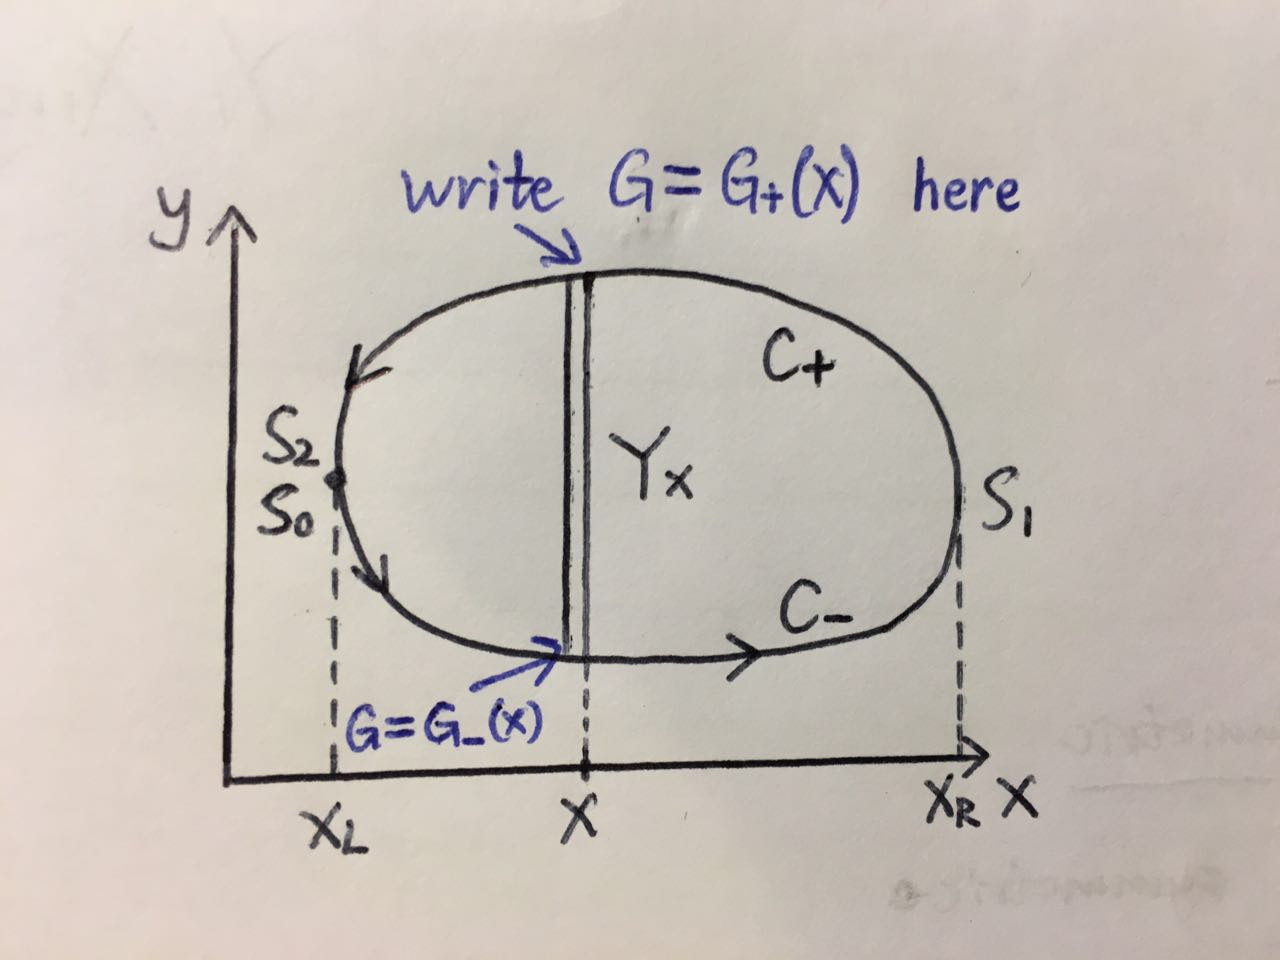
\includegraphics[scale=0.20]{VC01}\\
Recall 2D-Gauss theorem:\\
\begin{equation*}
\begin{aligned}
\int_A \nabla\cdot\mathbf{G}dA = \int_{C=\partial A} \mathbf{G}\cdot\mathbf{n}ds
\end{aligned}
\end{equation*}
Remark: $\int_C \mathbf{G}\cdot\mathbf{n}ds$ is different from $\int_C \mathbf{G}\cdot\mathbf{dr} = \int_C \mathbf{G}\cdot\mathbf{t}ds$ (e.g. as in Stokes' theorem).\\
\begin{equation*}
\begin{aligned}
\int_A \nabla\cdot\mathbf{G}dA &= \int_{x_L}^{x_R} \left(\int_{Y_x} \frac{\partial G}{\partial y}dy\right) dx\\
&= \int_{x_L}^{x_R} G_+ \left(x\right) - G_- \left(x\right) dx\\
&=\int_{x_L}^{x_R} G_+ \left(x\right)dx - \int_{x_L}^{x_R} G_- \left(x\right)dx
\end{aligned}
\end{equation*}
change variable to $s$ on $C_+$,i.e. opposite orientation to $x (S:R\to L)$ for the first integral, and change variable to $s$ on $C_-$, i.e. same orientation on $x(s:L\to R)$ for the second integral:
\begin{equation*}
\begin{aligned}
\int_{x_L}^{x_R} G_+ dx = \int_{S_2}^{S_1} G_+ \frac{dx}{ds} ds &= - \int_{C_+} \left(G_+ \frac{dx}{ds}\right) ds\\
\int_{x_L}^{x_R} G_- dx = \int_{S_0}^{S_1} G_- \frac{dx}{ds} ds &= - \int_{C_-} \left(G_- \frac{dx}{ds}\right) ds
\end{aligned}
\end{equation*}
Now relate $\frac{dx}{ds}$ 's to outward unit $\mathbf{n}$:\\
$\mathbf{t}=\left(\frac{dx}{ds},\frac{dy}{ds}\right)$ unit tangent;\\
$\mathbf{n}=\left(\frac{dy}{ds},-\frac{dx}{ds}\right)$ is the correct choice of signs to point outward.\\
vertical component of $\mathbf{n}$:\\
$\mathbf{j}\cdot\mathbf{n}=-\frac{dx}{ds}$ is positive on $C_+$, negative on $C_-$.\\
So
\begin{equation*}
\begin{aligned}
\int_{x_L}^{x_R} \left(G_+ - G_-\right) dx\\
&=-\int_{C_+} G\left(s\right) \frac{dx}{ds}ds - \int_{C_-} G\left(s\right) \frac{dx}{ds}ds\\
&=\int_{C_+} G \mathbf{j}\cdot\mathbf{n} ds + \int_{C_-} G \mathbf{j}\cdot\mathbf{n} ds\\
&=\int_C \mathbf{G}\cdot\mathbf{n}ds \text{  as  } \mathbf{G}=G\mathbf{j}.
\end{aligned}
\end{equation*}
For more general shapes, e.g.\\
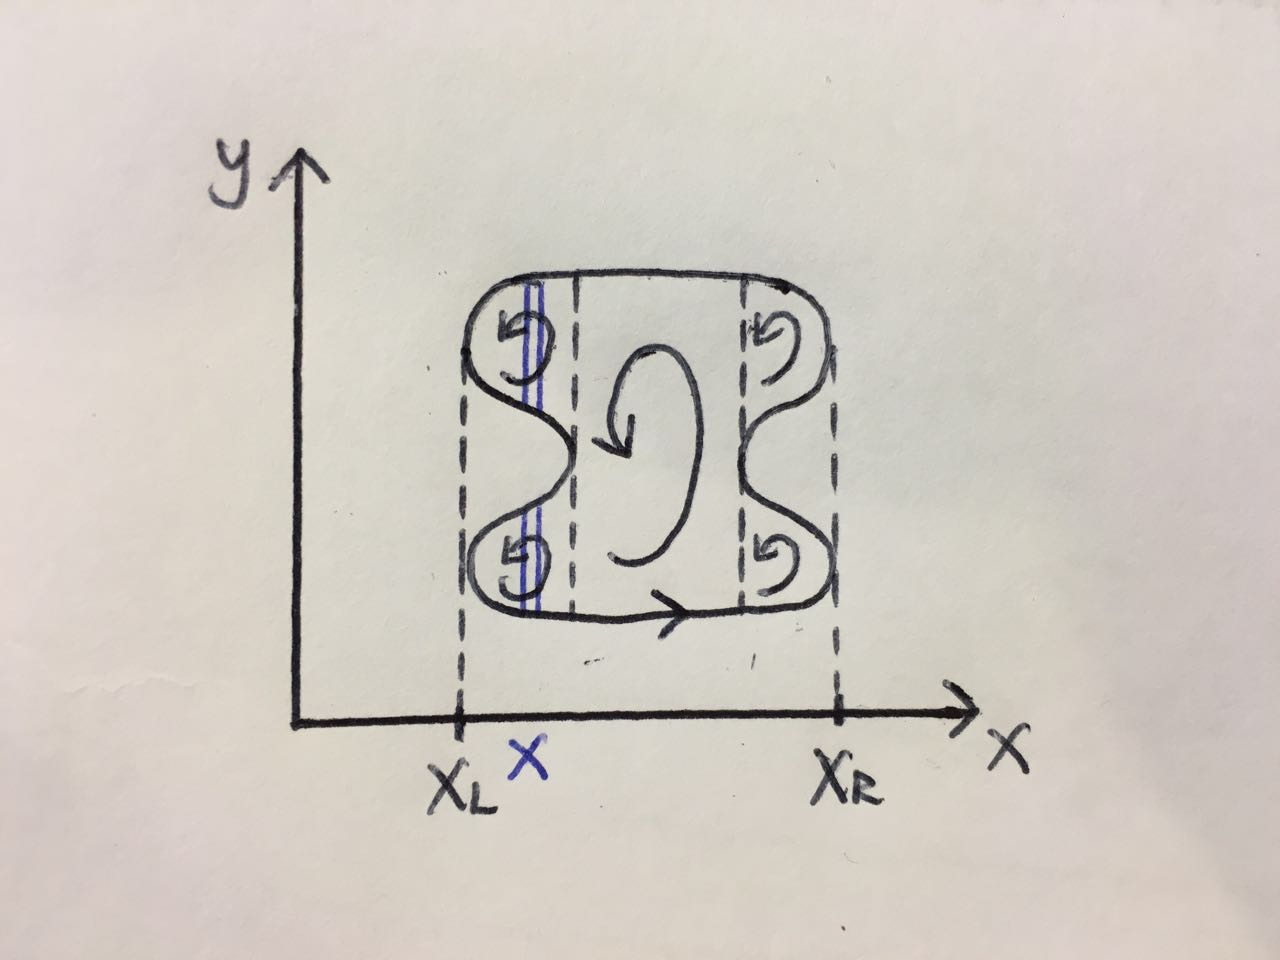
\includegraphics[scale=0.20]{VC02}\\
We either divide the region into simple pieces, and sum of all the dotted parts cancel;\\
or proceed as above with $Y_x$ now possibly a sum of intervals.\\
\begin{rem}
Same method can be used to prove 3D Gauss theorem: look at $\mathbf{G}$ of the form $\mathbf{G}=G\left(x,y,z\right)\mathbf{k}$ and vertical columns of volume for $\int_Y \vdiv \mathbf{G} dY$.
\end{rem}
(d) Green's theorem $\implies$ Stokes' theorem.\\
\begin{equation*}
\begin{aligned}
\int_S \left(\nabla\times\mathbf{F}\right)\cdot \mathbf{dS} = \int_{C=\partial S} \mathbf{F}\cdot\mathbf{dr}
\end{aligned}
\end{equation*}
$S$ and $C$ have consistent orientations.\\
Suppose $S$(the surface) is parameterised as $\mathbf{r}\left(u,v\right)$ for $\left(u,v\right)\in A\subseteq \R^2$.(Note that there are two different meanings of $S$ here: the surface, and the arclength of the boundary - kindly reminded by lecturer)\\
Then $\mathbf{dS}=\left(\frac{\partial \mathbf{r}}{\partial u}\times \frac{\partial\mathbf{r}}{\partial v}\right) dudv$.\\
and parameterised $\left(u,v\right)$ have fixed the orientation of $S$ ($\mathbf{n}$ in direction of $left(\frac{\partial \mathbf{r}}{\partial u}\times \frac{\partial\mathbf{r}}{\partial v}$).\\
So also fixed (consistent) orientation on $C\partial S$.\\
So 
\begin{equation*}
\begin{aligned}
\int_S \left(\nabla\times\mathbf{F}\right)\cdot\mathbf{ds}=\int_A \left(\nabla\times\mathbf{F}\right)\cdot\left(\frac{\partial \mathbf{r}}{\partial u}\times \frac{\partial\mathbf{r}}{\partial v}\right)dudv.
\end{aligned}
\end{equation*}
Fact:
\begin{equation*}
\begin{aligned}
\curl \mathbf{F}\left(\mathbf{r}\left(u,v\right)\right)\cdot \left(\frac{\partial \mathbf{r}}{\partial u}\times \frac{\partial\mathbf{r}}{\partial v}\right)\\
&= \frac{\partial \mathbf{F}}{\partial u}\cdot \frac{\partial \mathbf{r}}{\partial v}-\frac{\partial \mathbf{F}}{\partial v}\cdot \frac{\partial \mathbf{r}}{\partial u}.
\end{aligned}
\end{equation*}
Proof outline: just use suffix notation:
\begin{equation} \label{eq:2}
\begin{aligned}
LHS &= \left(\epsilon_{ijk} \frac{\partial F_j}{\partial x_i}\right)\left(\epsilon_{pqk} \frac{\partial x_p}{\partial u}\frac{\partial x_q}{\partial v}\right)
\end{aligned}
\end{equation}
Then use $\epsilon_{ijk}\epsilon_{pqk}=\delta_{ip}\delta_{jq}-\delta_{iq}\delta_{jp}$\\
and note:
\begin{equation*}
\begin{aligned}
\left(\frac{\partial \mathbf{F}}{\partial u}\right)_i &= \frac{\partial F_i}{\partial u}\\
&= \frac{\partial F_i}{\partial x_p}\frac{\partial x_p}{\partial u}\\
&= \frac{\partial F_i}{\partial x_j}\frac{\partial x_p}{\partial u}\delta_{jp}; \text{  Note the suffix notation used}\\
\left(\frac{\partial \mathbf{r}}{\partial v}\right)_i = \frac{\partial x_i}{\partial v}
\end{aligned}
\end{equation*}
substitute into (\ref{eq:2}) to get the result.\\

So we have
\begin{equation*}
\begin{aligned}
\partial_S \left(\nabla\times\mathbf{F}\right)\cdot\mathbf{dS}&=\int_A \left(\frac{\partial \mathbf{F}}{\partial u}\cdot\frac{\partial \mathbf{r}}{\partial v}-\frac{\partial \mathbf{F}}{\partial v} \cdot \frac{\partial \mathbf{r}}{\partial u}\right) dudv\\
&=\int_A \left[\frac{\partial}{\partial u}\left(\mathbf{F}\left(\mathbf{r}\left(u,v\right)\right)\cdot\frac{\partial \mathbf{r}}{\partial v}\right)-\frac{\partial}{\partial v}\left(\mathbf{F}\cdot\frac{\partial \mathbf{r}}{\partial u}\right)\right]dudv
\end{aligned}
\end{equation*}
Think Green!\\
for xy: 
\begin{equation*}
\begin{aligned}
\int_A \frac{\partial Q}{\partial x} - \frac{\partial P}{\partial y}dxdy = \int_C Pdx + Qdy \text{  anticlockwise}.
\end{aligned}
\end{equation*}
So Green's theorem in u-v plane gives:
\begin{equation*}
\begin{aligned}
\partial_S \left(\nabla\times\mathbf{F}\right)\cdot\mathbf{dS}=\int_C \left(\mathbf{F}\cdot\frac{\partial \mathbf{r}}{\partial u}\right)du + \left(\mathbf{F}\cdot\frac{\partial \mathbf{r}}{\partial v}\right)dv
\end{aligned}
\end{equation*}
Also along $C=\partial S \mathbf{dr} = \frac{\partial \mathbf{dr}}{\partial u}du + \frac{\partial \mathbf{r}}{\partial v}dv$,\\
So we get 
\begin{equation*}
\begin{aligned}
\int_S \left(\nabla\times\mathbf{F}\right)\cdot\mathbf{dS}=\int_C \mathbf{F}\cdot\mathbf{dr}.
\end{aligned}
\end{equation*}
Finally we should check that anti-clockwise orientation for $\partial A$ (needed in Green's theorem) agrees with the orientation of $\partial S$ imposed by the choice of parameters,i.e. $\mathbf{n}$ direction $~ \frac{\partial \mathbf{r}}{\partial u}\times\frac{\partial \mathbf{r}}{\partial v}$.\\
It always does! to see why:\\
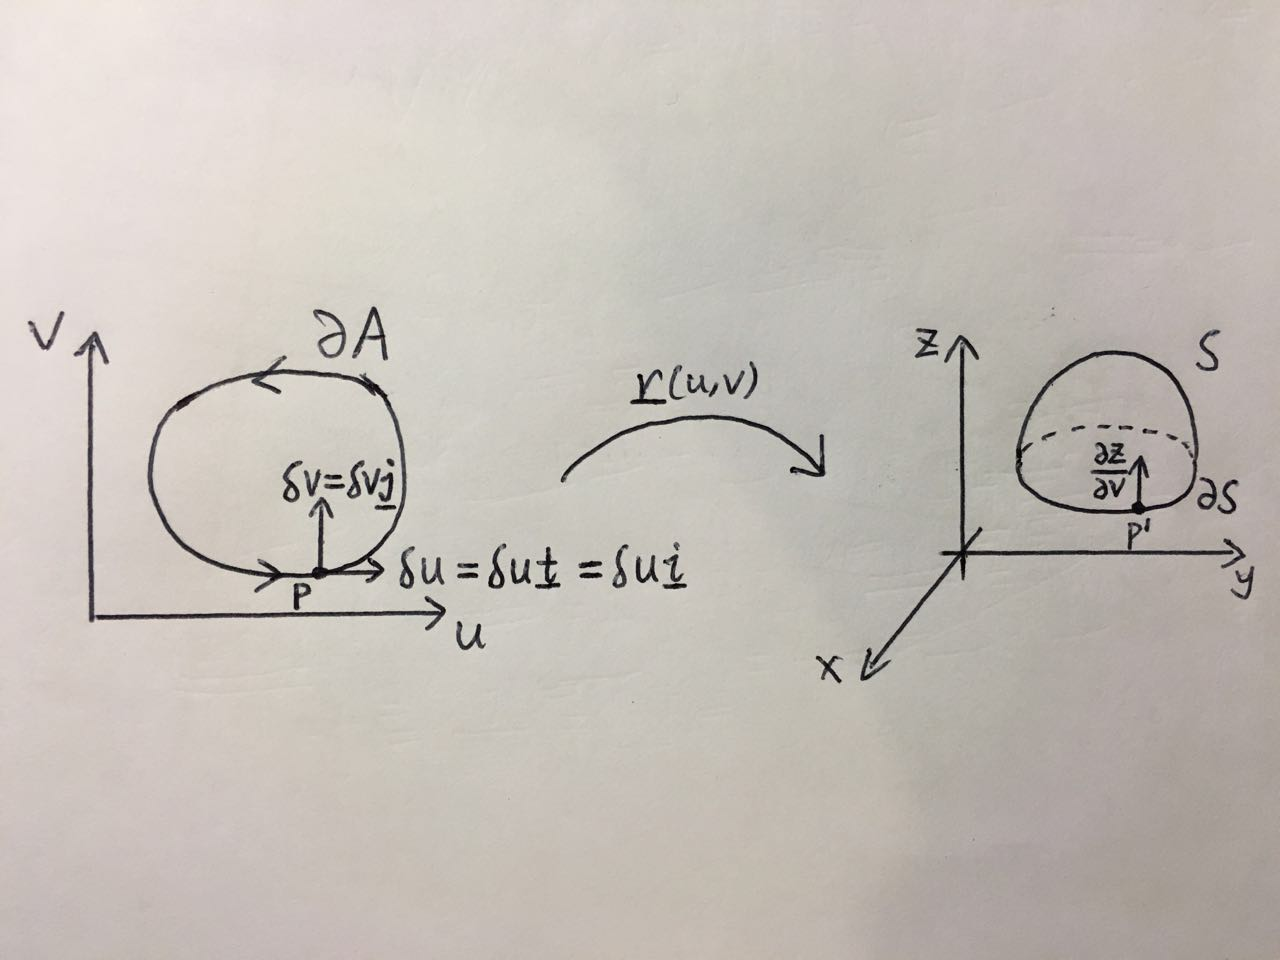
\includegraphics[scale=0.25]{VC03}\\
Consider $P$ on $\partial A$ where the tangent is parallel to the $u$ axis, mapping to $P'$ on $\partial S$.\\
Then small inward normal $\mathbf{\delta r}$ maps to $\mathbf{\delta r}\frac{\partial \mathbf{r}}{\partial v}\delta v$ must also point inward.\\
$\mathbf{\partial u}$ maps to $\mathbf{\partial r}$, tangent at $P_1$, can point to $L$ or $R$ on $\partial S$ \\
maps to $\frac{\partial \mathbf{r}}{\partial u}$ at $P'$.\\
=direction of traverse induced by anticlockwise on $\partial A$.\\
If points $L$ on $\partial S$ then $\mathbf{n} \sim \frac{\partial \mathbf{r}}{\partial u}\times\frac{\partial \mathbf{r}}{\partial v}$ points downwards (in picture) and consistent orientation on $\partial S$ is then to $L$.\\
If points $R$ then $\mathbf{n}$ points upwards, and consistent again.\\
\end{proof}

\newpage
\section{Geometrical characterisation of div and curl}
Apply divergence theorem to small volume $V$ (size $V$), containing $\mathbf{r}$:
\begin{equation*}
\begin{aligned}
\int_{\partial V} \mathbf{F}\cdot \mathbf{dS} = \int_V \nabla\cdot\mathbf{F}dV \approx \nabla\cdot\mathbf{F}|_\mathbf{r} V
\end{aligned}
\end{equation*}
This becomes exact as $V\to 0$:
\begin{equation}\label{eq:3}
\begin{aligned}
\vdiv \mathbf{F} = \lim_{V\to 0} \frac{1}{V} \int_{\partial V} \mathbf{F}\cdot \mathbf{dS}
\end{aligned}
\end{equation}
Similarly, Stoke's theorem for small planar surface $S$ (area $S$) containing $\mathbf{r}$, unit normal $\mathbf{n}$:
\begin{equation*}
\begin{aligned}
\int_{\partial S} \mathbf{F}\cdot\mathbf{dr} &= \int_S \left(\nabla\times\mathbf{F}\right)\cdot\mathbf{n} dS\\
&= \mathbf{n}\cdot\nabla\times\mathbf{F} S
\end{aligned}
\end{equation*}
so
\begin{equation}\label{eq:4}
\begin{aligned}
\mathbf{n}\cdot\nabla\times\mathbf{F}=\lim_{S\to 0} \frac{1}{S} \int_{\partial S} \mathbf{F}\cdot\mathbf{dr}
\end{aligned}
\end{equation}

(\ref{eq:3}) and (\ref{eq:4}) manifestly coordinates independent -- purely geometrical.\\
This could be used as definitions. Then Stoke's and Gauss' theorems become easy to prove.\\

\begin{eg} (Stoke's theorem)\\
Divide $S$ up into many small loops:\\
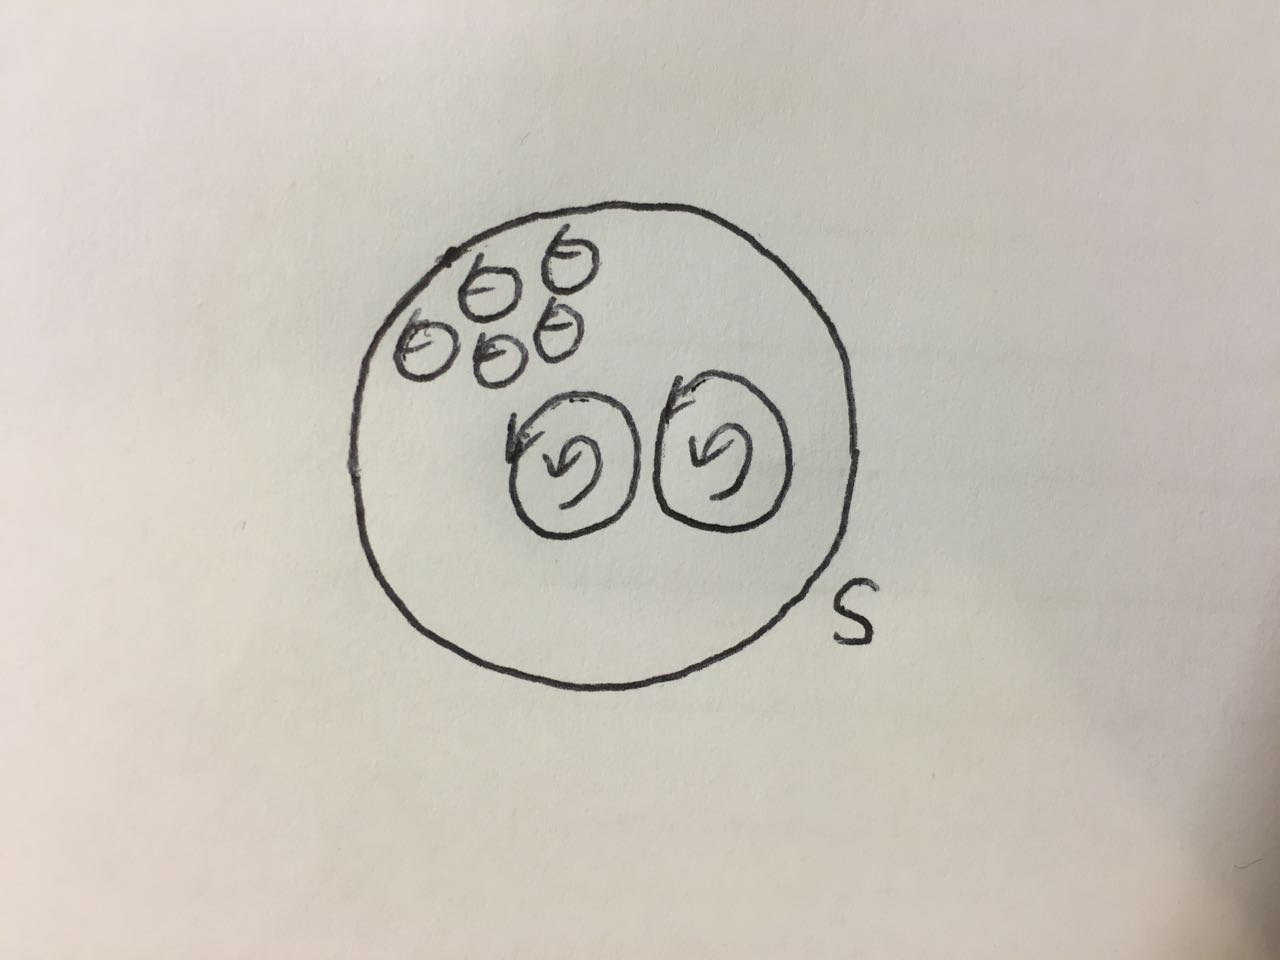
\includegraphics[scale=0.15]{VC04}\\
By (\ref{eq:4}), $\int \left(\nabla\times\mathbf{F}\right)\cdot\mathbf{n}dS = $ sum of all circulations of $\mathbf{F}$, all anticlockwise(or all clockwise); where adjacent loop contact, circulations cancel since directions opposite.\\
Hence sum of circulations all cancel except at the boundary where there is no matching adjacent loop. The result is simply the circulation on the boundary, i.e. $\int_C \mathbf{F}\cdot\mathbf{dr}$.
\end{eg}

\begin{eg} (Gauss' theorem)\\
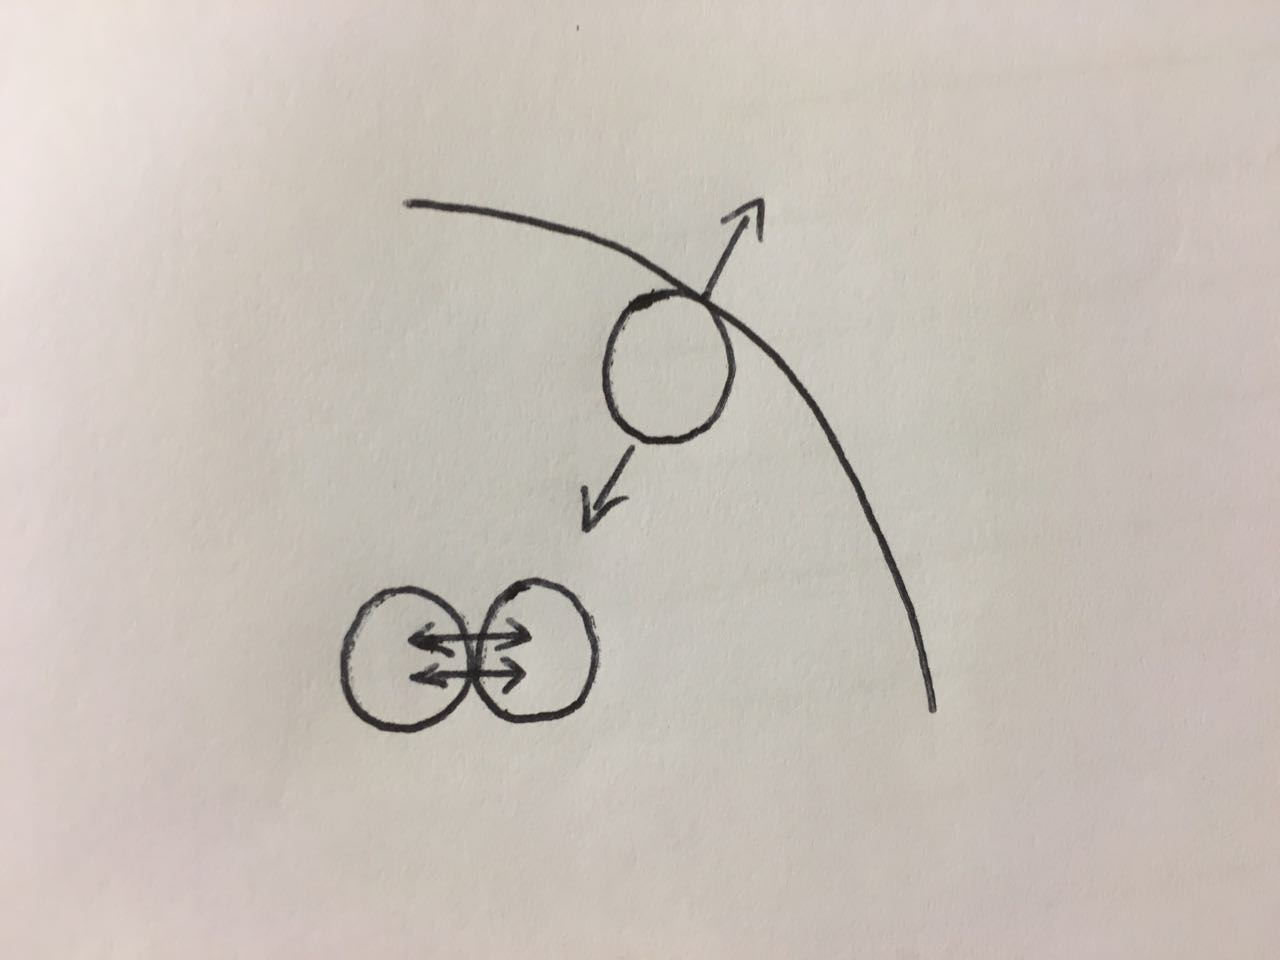
\includegraphics[scale=0.15]{VC05}\\
Similarly the outward flows from all small regions cancel on all internal surface contacts, leaving only outward flow on boundary, i.e. $\int_V \vdiv\mathbf{F}dV = \int_{\partial V} \mathbf{F}\cdot\mathbf{n}dS$.\\
\end{eg}

\begin{eg} (Fluid dynamics)\\
Let $\mathbf{u}$ be velocity field of a fluid flow in 3D.\\
For div: had before $\int_S \mathbf{u}\cdot\mathbf{dS}$ is rate of fluid crossing surface.\\
For closed surface (and outward $\mathbf{n}$) it is the total outflow from $S$ per unit time.\\
So $\vdiv \mathbf{u}$ is the outflow rate per unit volume for small local volumes (as volume $\to$ 0).\\
If the density of fluid is constant, i.e. flow is incompressible, then must have $\vdiv \mathbf{u}=0$ (assuming no cavities develop).\\
Above is for a fixed volume $V$. We can also consider moving volumes: consider fluid 'particles' in $V$ at time, moving for time $\delta t$ (small), under the flow they occupy new positions and get new volumes.\\
Small surface element $\mathbf{dS}$ moves through $\mathbf{u}\delta t$ appending extra volume $\mathbf{\delta S}\cdot\mathbf{u}\delta t$ to $V$.\\
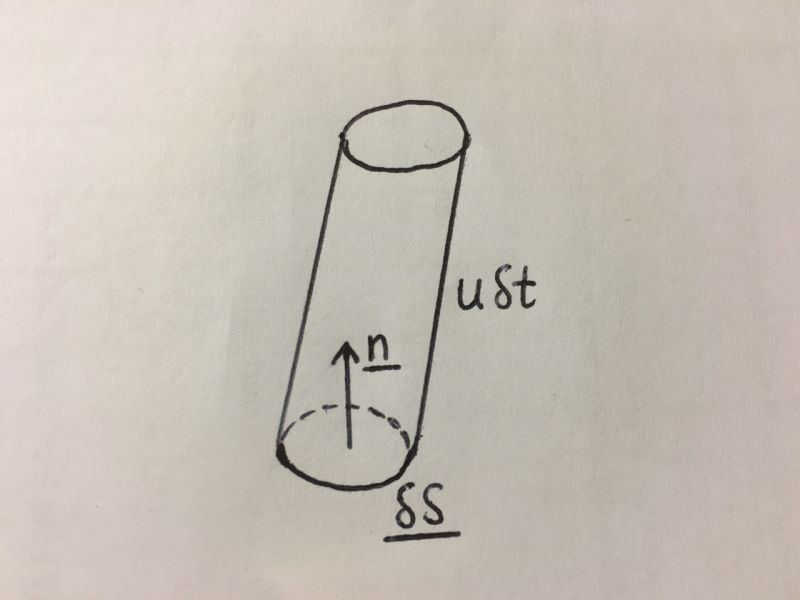
\includegraphics[scale=0.15]{VC06}\\
So summing over whole surface:
\begin{equation*}
\begin{aligned}
V\left(t+\delta t\right)-v\left(t\right)=\delta V = \sum \mathbf{\delta S}\cdot \mathbf{u}\delta t \text{  + o terms}.
\end{aligned}
\end{equation*}
In limit as $\delta t\to 0, \delta S$'s $\to 0$:
\begin{equation*}
\begin{aligned}
\frac{dV}{dt} = \int_S \mathbf{u}\cdot\mathbf{dS}=\int_V \vdiv \mathbf{u} dV
\end{aligned}
\end{equation*}
So for small volumes around a point $\mathbf{r}$ get $\vdiv \mathbf{u}=\frac{1}{V}\dot{V}$ (rate of change of volume per unit volume).\\
If you "go with the flow":\\
Again incompressibility = volume is preserved, i.e. $\vdiv \mathbf{u}=0$.

For curl:\\
Let $A$ be planar disc, centre $\mathbf{r}$, radius $a$, normal $\mathbf{n}$:\\
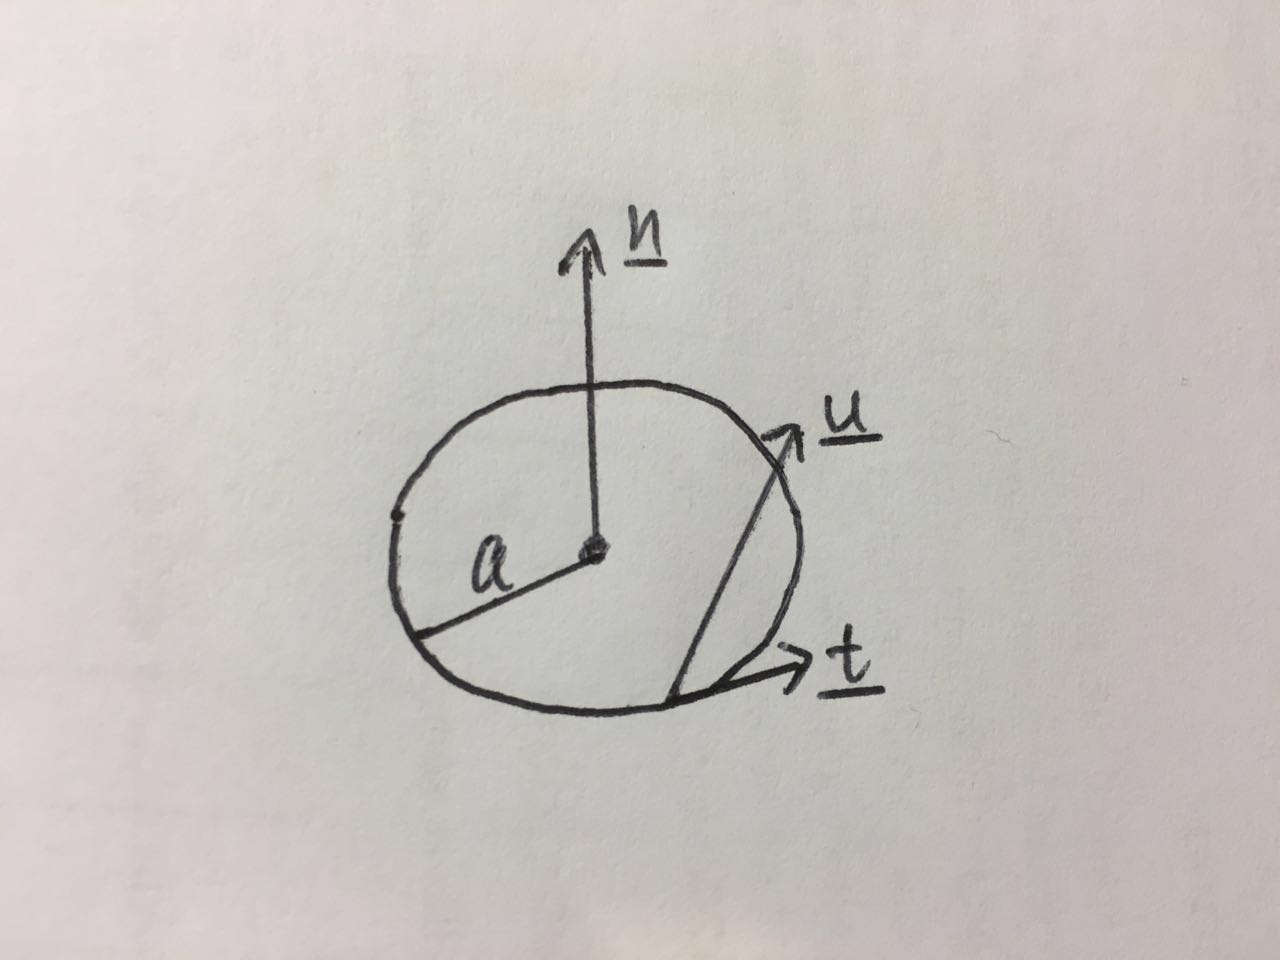
\includegraphics[scale=0.15]{VC07}\\
then
\begin{equation*}
\begin{aligned}
\int_{\partial A} \mathbf{u}\cdot\mathbf{dr} &= \int_{\partial A} \mathbf{u}\cdot\mathbf{t} dS\\
&= 2\pi a \cdot (\text{average tengential component of }\mathbf{u}, \text{write as }\overline{u}_{tang})\\
&= 2\pi a^2 \omega
\end{aligned}
\end{equation*}
where $\omega = \frac{1}{a} \bar{u}_{tang}$ is the angular velocity. corresponding $\bar{u}_{tang}$ speed at radius $a$.\\
Then by (\ref{eq:4})
\begin{equation*}
\begin{aligned}
\mathbf{n}\cdot\nabla\times\mathbf{u}=\lim_{a\to 0} \frac{1}{\pi a^2} 2\pi a^2 \omega = 2\omega
\end{aligned}
\end{equation*}
i.e. $\left(\curl \mathbf{u}\right)\cdot\mathbf{n}=$twice local rate of rotation of fluid near $\mathbf{r}$.\\
$\bar{u}_{tang}$ is independent of overall motion $\mathbf{u}\to\mathbf{u} + $\underline{constant} as $\bar{const}_{tang} = 0$.
\end{eg}

\newpage
\section{Conservation laws}
For space and time dependent scalar and vector fields $\rho\left(\mathbf{r},t\right),\mathbf{j}\left(\mathbf{r},t\right)$:
\begin{equation}\label{eq:5}
\begin{aligned}
\frac{\partial p}{\partial t}+\nabla\cdot\mathbf{j}=0
\end{aligned}
\end{equation}
is called the \emph{conservation equation}(or continuity equation).\\
Why? -- let $V$ be fixed volume in space, boundary $S=\partial V$. Then
\begin{equation*}
\begin{aligned}
Q\left(t\right)=\int_V \rho\left(\mathbf{r},t\right) dV
\end{aligned}
\end{equation*}
satisfies
\begin{equation}\label{eq:6}
\begin{aligned}
\frac{dQ}{dt}&=\int_V \frac{\partial \rho}{\partial t} dV\\
&= -\int_V \vdiv \mathbf{j}dV\\
&= -\int_S \mathbf{j}\cdot\mathbf{dS}
\end{aligned}
\end{equation}
If we think of $\rho$ as density of some quantity $q$(mass, charge,...) and $\mathbf{j}$ is the current density for it, i.e. for any small surface element $\mathbf{dS}$ in space,\\
$\mathbf{j}\cdot\mathbf{dS}=$amount of $q$ crossing $\mathbf{dS}$ per unit time (flux of $q$ across $\mathbf{dS}$).\\
Then $\mathbf{Q}\left(t\right)$ = total amount of $q$ in $V$, and (\ref{eq:6}) expresses conservation of $q$, in the sense that any change of amount of $q$ in $V$ must be associated to the same amount of $Q$ passing across the boundary of $\partial V$.\\
Equivalently (\ref{eq:5}) expresses conservation of $q$ (for any $V$).\\
$\bullet$ more than just overall conservation -- it imposes local conservation.\\
eg.\\
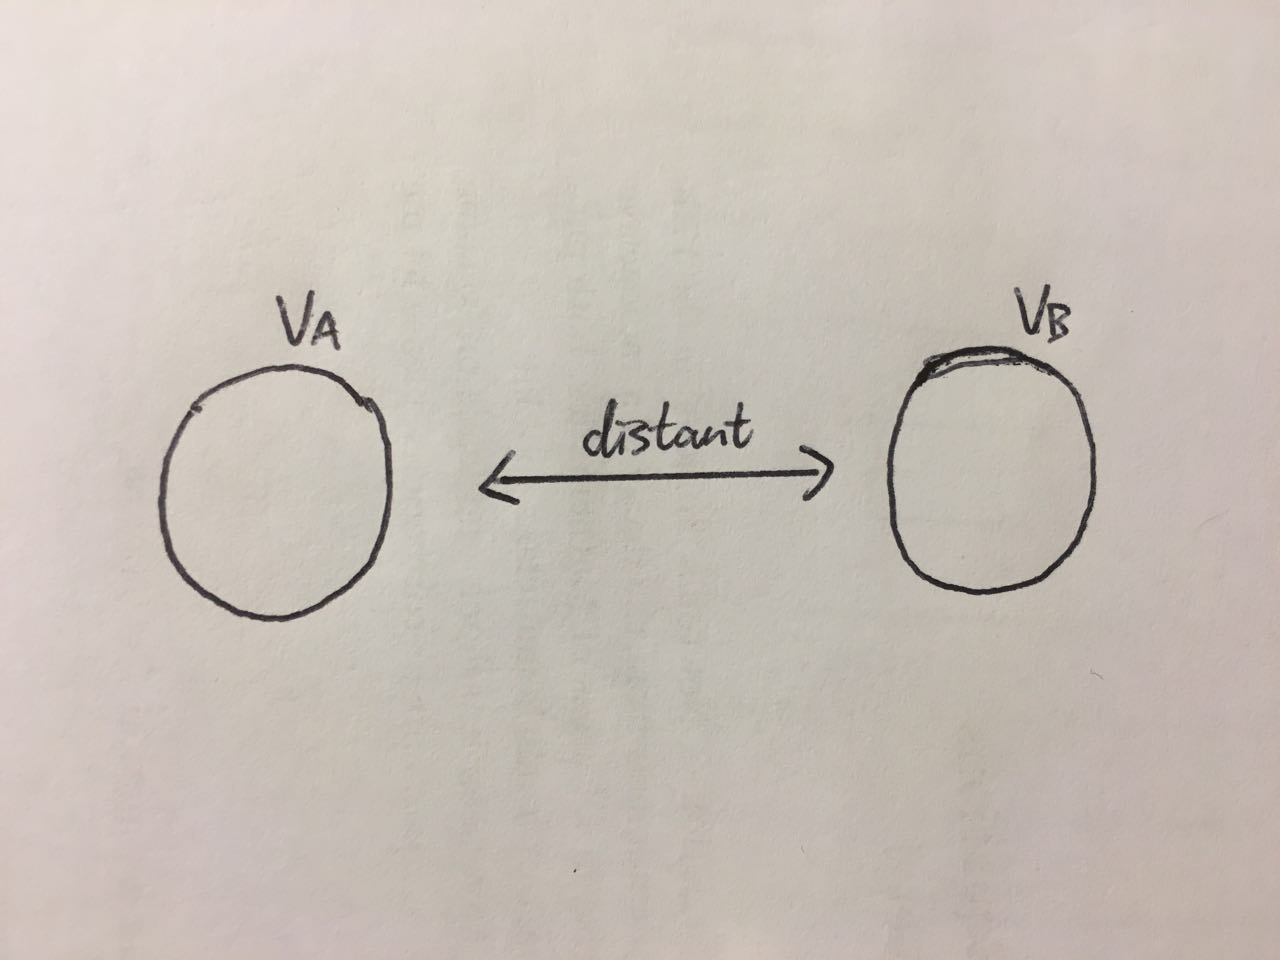
\includegraphics[scale=0.15]{VC08}\\
Cannot have $q$ decreasing in $V_A$ while increasing in distant $V_B$ by same amount (so $q$ is conserved overall) but nothing happening in between.\\
Decrease in $V_A$ can only happen if some $q$ flows out across its boundary.\\

\begin{eg}
1) conservation of electric charge:\\
$\rho\left(\mathbf{r},t\right) \sim$ charge density;\\
$\mathbf{j}\left(\mathbf{r},t\right) \sim$ electric current density.\\

2) conservation of mass for fluid motion:\\
$\rho\left(\mathbf{r},t\right) \sim$ mass density;\\
$\mathbf{j}=\rho\mathbf{u}$ is mass current if $\mathbf{u}$ is the velocity field.\\
Volume $\delta V \sim \mathbf{n}\cdot\mathbf{u}\delta t\delta S$. So mass $\sim \rho\mathbf{n}\cdot\mathbf{u}\delta t\delta S$.\\
So $\frac{\partial \rho}{\partial t}+\vdiv\left(\rho\mathbf{u}\right)=0$ for fluid motion.\\
If $\rho$ is also constant, get $\vdiv\left(\mathbf{u}\right)=0$.\\
\end{eg}

We know $\mathbf{F}$ is conservative $\left(\mathbf{F}=\nabla f\right) \implies \mathbf{F}$ is irrotational ($\nabla \times \mathbf{F}=\mathbf{0}$).\\
Now proved converse: suppose $\mathbf{F}$ is irrotational on a simply connected region $D\subseteq \R^3$.\\
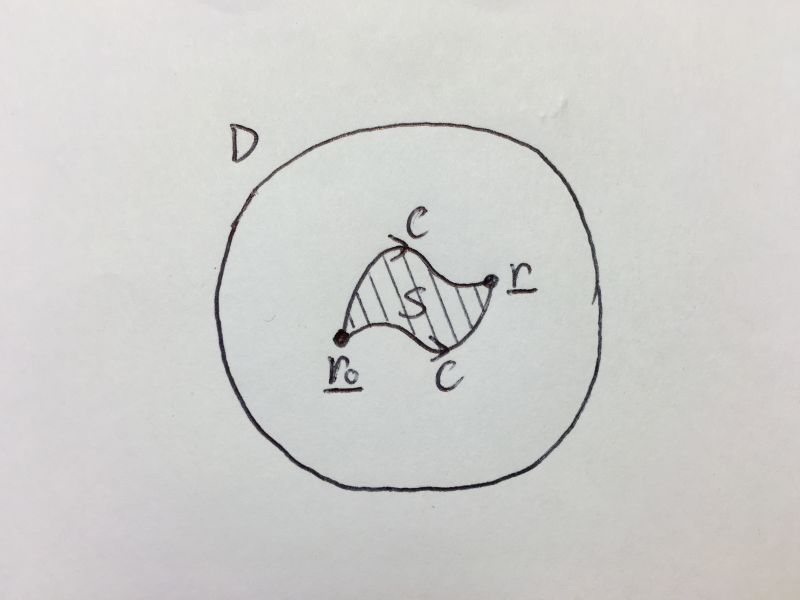
\includegraphics[scale=0.15]{VC09}\\
For any fixed $\mathbf{r_0} \in D$ and variable $\mathbf{r}$, consider\\
\begin{equation*}
\begin{aligned}
f\left(\mathbf{r}\right) = \int_C \mathbf{F}\cdot \mathbf{dr}
\end{aligned}
\end{equation*}
For a choice of curve $C$ from $\mathbf{r_0}$ to $\mathbf{r}$.\\
This is independent of choice of $C$ by Stoke's theorem:\\
If $C'$ is any other curve, it can be smoothly deformed into $C$, defining a spanning surface $S$.\\
If while $\partial S$ oriented in direction of $C$ (so opposite on $C'$), then Stoke's theorem implies
\begin{equation*}
\begin{aligned}
\int_S \nabla\times\mathbf{F}\cdot\mathbf{ds} &= \int_C \mathbf{F}\cdot\mathbf{dr} - \int_{C'} \mathbf{F}\cdot\mathbf{dr}
\end{aligned}
\end{equation*}
But $\nabla \times \mathbf{F}=\mathbf{0}$, so the two integrals are equal.\\
Hence $f\left(\mathbf{r}\right)$ is well defined on all $D$.\\

Claim: $\mathbf{F}=\nabla f$.\\
Consider extending $C$ by a small $\mathbf{\delta r}$ at $\mathbf{r}$ giving $C+\delta C$:\\
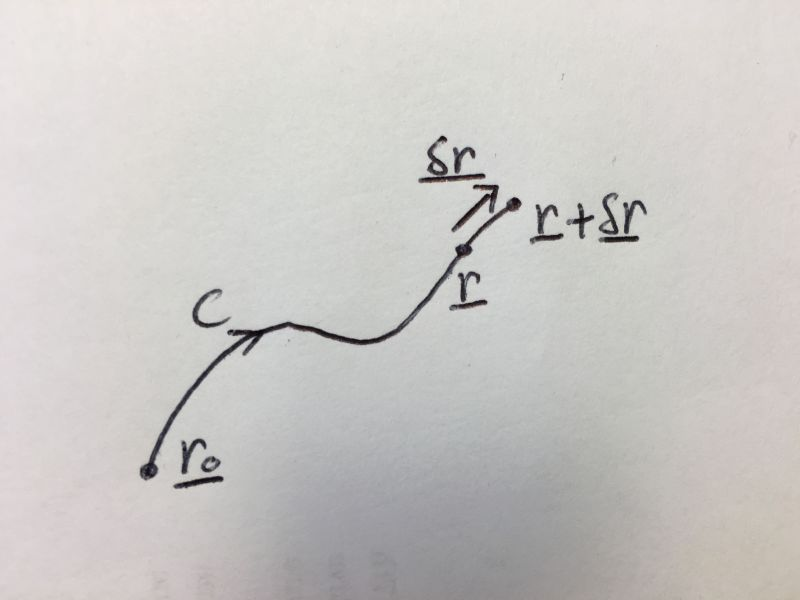
\includegraphics[scale=0.15]{VC10}\\
\begin{equation*}
\begin{aligned}
f\left(\mathbf{r}+\mathbf{\delta r}\right) &= \int_{C+\delta C} \mathbf{F}\cdot\mathbf{dr}\\
&= \int_C \mathbf{F}\cdot\mathbf{dr} + \int_{\delta C} \mathbf{F}\cdot \mathbf{dr}\\
&=f\left(\mathbf{r}\right)+\mathbf{F}\left(\mathbf{r}\right)\cdot\mathbf{\delta r} + o\left(|\mathbf{\delta r}|\right)
\end{aligned}
\end{equation*}
So
\begin{equation*}
\begin{aligned}
\delta f &= \mathbf{F}\left(\mathbf{r}\right)\cdot\mathbf{\delta r} + \text{ o terms}
\end{aligned}
\end{equation*}
But by definition of $\nabla f$,
\begin{equation*}
\begin{aligned}
\delta f = \nabla f \cdot \mathbf{\delta r} + \text{ o terms}
\end{aligned}
\end{equation*}
So $\mathbf{F}=\nabla f.$\\

\newpage
\section{Orthogonal curvilinear coordinates}
Consider coordinates $\left(u,v,w\right)$ on $\R^3$, and small invertible functions $\mathbf{r}\left(u,v,w\right)$.\\

\subsection{Line element, surface element, volume element}
Line element is
\begin{equation*}
\begin{aligned}
\mathbf{dr}&=\frac{\partial \mathbf{r}}{\partial u}du + \frac{\partial \mathbf{r}}{\partial v}dv + \frac{\partial \mathbf{r}}{\partial w}dw
\end{aligned}
\end{equation*}
Here $\frac{\partial \mathbf{r}}{\partial u},\frac{\partial \mathbf{r}}{\partial v},\frac{\partial \mathbf{r}}{\partial w}$ are tangent to coordinate lines of $u,v,w$ respectively (since the other two are hold constant).\\
Require these to be linearly independent,i.e.:
\begin{equation*}
\begin{aligned}
\frac{\partial \mathbf{r}}{\partial u}\cdot\left(\frac{\partial \mathbf{r}}{\partial v}\times\frac{\partial \mathbf{r}}{\partial w}\right) \neq 0.
\end{aligned}
\end{equation*}
(also equal to the \emph{Jacobian}, $\frac{\partial \left(x,y,z\right)}{\partial \left(u,v,w\right)}$).\\
$\left(u,v,w\right)$ are \emph{orthogonal} curvilinear coordinates.\\
If $\frac{\partial \mathbf{r}}{\partial u},\frac{\partial \mathbf{r}}{\partial v},\frac{\partial \mathbf{r}}{\partial w}$ are orthogonal vectors, then set
\begin{equation}\label{eq:7}
\begin{aligned}
\frac{\partial \mathbf{r}}{\partial u} &= h_u\mathbf{e}_u\\
\frac{\partial \mathbf{r}}{\partial v} &= h_u\mathbf{e}_v\\
\frac{\partial \mathbf{r}}{\partial w} &= h_u\mathbf{e}_w
\end{aligned}
\end{equation}
with $h_u,h_v,h_w$ all greater than 0, and $\mathbf{e}_u,\mathbf{e}_v,\mathbf{e}_w$ are orthonormal and form a right-handed system, i.e. $\mathbf{e}_u\times \mathbf{e}_v = \mathbf{e}_w$ etc. This can always be achieved by re-ordering coordinates appropriately.\\
Then the \emph{line element} is
\begin{equation}\label{eq:8}
\begin{aligned}
\mathbf{dr} &= h_u\mathbf{e}_u du + h_v\mathbf{e}_v dv + h_w\mathbf{e}_w dw
\end{aligned}
\end{equation}
So the square of distance induced by small changes in $u,v,w$ is (up to o-terms):
\begin{equation*}
\begin{aligned}
|\mathbf{\delta r}|^2 &= h_u^2\delta u^2+h_v^2\delta v^2+h_w^2\delta w^2
\end{aligned}
\end{equation*}
So $h_u,h_v,h_w$ are positive scale factors for distance along the curve.\\

For surface elements:\\
Consider co-ordinate surfaces $w=$constant, parameterised by $u,v$.\\
Area element,
\begin{equation*}
\begin{aligned}
\mathbf{dS} &= \left(\frac{\partial \mathbf{r}}{\partial u}\times \frac{\partial \mathbf{r}}{\partial v}\right) dudv \text{  (general formula)}\\
&= h_u\mathbf{e}_u\times h_v\mathbf{e}_v dudv\\
&= h_u h_v \mathbf{e}_w dudv \text{  (for orthogonal coordinates)}
\end{aligned}
\end{equation*}
Geometrically, $dS$ is a small rectangle of side lengths $h_u \delta u$ and $h_v \delta v$ with normal $\mathbf{e}_w$.\\
Similarly, for surface elements of $u=$constant and $v=$ constant surfaces.\\

For volume elements:\\
The Jacobian formula gives
\begin{equation*}
\begin{aligned}
dV&=\frac{\partial \mathbf{r}}{\partial u}\cdot\left(\frac{\partial \mathbf{r}}{\partial v}\times\frac{\partial\mathbf{r}}{\partial w}\right)dudvdw\\
&=h_u h_v h_w dudvdw
\end{aligned}
\end{equation*}
($\sim$ small cuboid with sides $h_u\delta u,h_v\delta v,h_w\delta w$).\\

\subsection{Grad, div and curl in curvilinear coordinates}
Coordinate-independent definition of $\grad$ is
\begin{equation*}
\begin{aligned}
df &= \nabla f \cdot \mathbf{dr}
\end{aligned}
\end{equation*}
for any scalar function $f$. But also
\begin{equation*}
\begin{aligned}
df &= \frac{\partial f}{\partial u}du + \frac{\partial f}{\partial v}dv + \frac{\partial f}{\partial w}dw.
\end{aligned}
\end{equation*}
Substitute (\ref{eq:8}) for $\mathbf{dr}$ above, compare coefficients of $du,dv,dw$ and get
\begin{equation*}
\begin{aligned}
\nabla f &=\frac{1}{h_u}\mathbf{e}_u \frac{\partial f}{\partial u} +\frac{1}{h_v}\mathbf{e}_v \frac{\partial f}{\partial v} +\frac{1}{h_w}\mathbf{e}_w \frac{\partial f}{\partial w}
\end{aligned}
\end{equation*}
expressing $\grad$ in curvilinear coordinates.\\
(For both the variables and unit vectors for components)\\

For vector field 
\begin{equation*}
\begin{aligned}
\mathbf{F} = F_u \mathbf{e}_u + F_v \mathbf{e}_v + F_w \mathbf{e}_w
\end{aligned}
\end{equation*}
in $\left(u,v,w\right)$ system,
$\vdiv \mathbf{F}$ and $\curl \mathbf{F}$ are more complicated as $\mathbf{e}_u,\mathbf{e}_v,\mathbf{e}_w$ are generally \emph{not} constant now.\\

Several ways to derive formulas:\\
e.g. use coordinate-independent formulas for $\nabla \cdot \mathbf{F},\nabla \times \mathbf{F}$ or algebraic methods, get (derivations not part of the course):
\begin{equation*}
\begin{aligned}
\nabla \times \mathbf{F}&=\frac{1}{h_u h_v h_w}
\begin{vmatrix}
h_u \mathbf{e}_u & h_v \mathbf{e}_v & h_w \mathbf{e}_w\\
\frac{\partial}{\partial u} & \frac{\partial}{\partial v} & \frac{\partial}{\partial w}\\
h_u F_u & h_v F_v & h_w F_w
\end{vmatrix}\\
&= \frac{1}{h_v h_w}[\frac{\partial}{\partial v}\left(h_w F_w\right)-\frac{\partial}{\partial w}\left(h_v F_v\right)]\mathbf{e}_u + \text{  (two similar terms)},\\
\nabla \cdot \mathbf{F} &= \frac{1}{h_u h_v h_w}[\frac{\partial}{\partial u}\left(h_v h_w F_u\right)+ \text{  (two similar terms)]}.
\end{aligned}
\end{equation*}

\begin{eg}
\begin{equation*}
\begin{aligned}
\mathbf{A} &= \frac{1}{r}\tan\frac{\theta}{2}\mathbf{e}_\varphi
\end{aligned}
\end{equation*}
in spherical polar coordinates.
\begin{equation*}
\begin{aligned}
h_r = 1, h_\theta = 1, h_\varphi = r\sin\theta
\end{aligned}
\end{equation*}
So
\begin{equation*}
\begin{aligned}
\nabla\times\mathbf{A} &= \frac{1}{r^2 \sin\theta}
\begin{vmatrix}
\mathbf{e}_r & r\mathbf{e}_\theta & r\sin\theta\mathbf{e}_\varphi\\
\frac{\partial}{\partial r} & \frac{\partial}{\partial \theta} & \frac{\partial}{\partial \varphi}\\
0 & 0 & r\sin\theta \cdot \frac{1}{r} \tan \frac{\theta}{2}
\end{vmatrix}\\
&= \frac{1}{r^2 \sin\theta} \mathbf{e}_r \frac{\partial}{\partial \theta} \left(2 \sin^2 \frac{\theta}{2}\right)\\
&= \frac{1}{r^2} \mathbf{e}_r
\end{aligned}
\end{equation*}
\end{eg}

\begin{eg} (Algebraic method for $\curl$ and $\vdiv$ formula (outline)\\
$\bullet$ for $\curl$:\\
Note first 
\begin{equation*}
\begin{aligned}
\nabla\times\left(\frac{\mathbf{e}_u}{h_u}\right)=0
\end{aligned}
\end{equation*}
since
\begin{equation*}
\begin{aligned}
\nabla u = \frac{\mathbf{e}_u}{h_u} \text{  and  } \curl\grad = 0
\end{aligned}
\end{equation*}
Similarly
\begin{equation*}
\begin{aligned}
\nabla\times\left(\frac{\mathbf{e}_v}{h_v}\right)=\nabla\times\left(\frac{\mathbf{e}_w}{h_w}\right)=0
\end{aligned}
\end{equation*}
Now for $\nabla\times\mathbf{F}$, write
\begin{equation*}
\begin{aligned}
\mathbf{F} &= F_u \mathbf{e}_u+F_v \mathbf{e}_v+F_w \mathbf{e}_w\\
&=F_u h_u \left(\frac{\mathbf{e}_u}{h_u}+F_v h_v\right) +\left(\frac{\mathbf{e}_v}{h_v}\right)+F_w h_w \left(\frac{\mathbf{e}_w}{h_w}\right)
\end{aligned}
\end{equation*}
Then recall
\begin{equation*}
\begin{aligned}
\nabla\times\left(q\mathbf{V}\right)=\nabla\varphi\times\mathbf{V}+\varphi\left(\nabla\times\mathbf{V}\right)
\end{aligned}
\end{equation*}
So
\begin{equation*}
\begin{aligned}
\nabla\times\mathbf{F}=\nabla\left(F_u h_u\right)\times\frac{\mathbf{e}_u}{h_u}+\nabla\left(F_v h_v\right)\times\frac{\mathbf{e}_v}{h_v}+\nabla\left(F_w h_w\right)\times\frac{\mathbf{e}_w}{h_w}
\end{aligned}
\end{equation*}
\end{eg}

$\bullet$ for $\vdiv$:\\
Starting trick is to note
\begin{equation}\label{eq:9}
\begin{aligned}
\vdiv\left(\frac{\mathbf{e}_w}{h_u h_v}\right)=\vdiv\left(\frac{\mathbf{e}_v}{h_u h_w}\right)=\vdiv\left(\frac{\mathbf{e}_u}{h_v h_w}\right)=0
\end{aligned}
\end{equation}
because
\begin{equation*}
\begin{aligned}
\frac{\mathbf{e}_u}{h_u}=\nabla u,\frac{\mathbf{e}_v}{h_v}=\nabla v,\frac{\mathbf{e}_w}{h_w}=\nabla w
\end{aligned}
\end{equation*}
So
\begin{equation*}
\begin{aligned}
\frac{\mathbf{e}_w}{h_u h_v} = \nabla u \times \nabla v
\end{aligned}
\end{equation*}
and
\begin{equation*}
\begin{aligned}
\nabla\cdot\left(\mathbf{A}\times\mathbf{B}\right) = \mathbf{B}\cdot\left(\nabla\times \mathbf{A}\right)-\mathbf{A}\cdot\left(\nabla\times\mathbf{B}\right)
\end{aligned}
\end{equation*}
again get (\ref{eq:9}) by $\curl\grad = 0$.\\
Then write
\begin{equation*}
\begin{aligned}
\mathbf{F}=F_u h_v h_w \left(\frac{\mathbf{e}_u}{h_v h_w}\right) + \text{  two similar terms}
\end{aligned}
\end{equation*}
and use
\begin{equation*}
\begin{aligned}
\vdiv\left(\varphi\mathbf{F}\right) = \varphi\left(\nabla\cdot\mathbf{V}\right)+\mathbf{V}\cdot\left(\nabla\varphi\right).
\end{aligned}
\end{equation*}

\newpage
\section{Laplace equation and Poisson equation}

\subsection{Gauss' Law and Poisson equation}
Consider gravitational force $\mathbf{F}\left(\mathbf{r}\right)$ on point mass $m$ at $\mathbf{r}$, from some distribution of mass in space.\\
Write 
\begin{equation*}
\begin{aligned}
\mathbf{F}\left(\mathbf{r}\right)=m\mathbf{g}\left(\mathbf{r}\right)
\end{aligned}
\end{equation*}
$\mathbf{g}\left(\mathbf{r}\right)$ is the gravitational field/force per unit mass/acceleration due to gravity.\\

\begin{thm} (Gauss' law in integral form)\\
relates $\mathbf{g}$ to mass distribution
\begin{equation*}
\begin{aligned}
\int_S \mathbf{g}\cdot\mathbf{dS}=-4\pi GM
\end{aligned}
\end{equation*}
for any closed surface $S$, bounding a volume $V$.\\
$M$ is the total mass contained in $V$. $G$ is the Newtonian gravitational constant.
This can be used as the law of gravitation:\\
$\bullet$ Newton inverse square law follows from Gauss (plus an extra symmetry assumption);\\
$\bullet$ Gauss follow from Newton too (in Part 1B Methods -- Green's functions for PDE, $\delta$-functions).
\end{thm}

To get Newton from Gauss:\\
Consider total mass $M$, distributed with spherical symmetry about $\mathbf{0}$, all contained in sphere radius $a$.\\
Assume that spherical symmetry $\implies$ $\mathbf{g}\left(\mathbf{r}\right)$ is radial,
\begin{equation*}
\begin{aligned}
\mathbf{g}\left(\mathbf{r}\right) = g\left(\mathbf{r}\right)\mathbf{e}_r
\end{aligned}
\end{equation*}
Now apply Gauss law for $S$ = a sphere of radius $R>a$.
\begin{equation*}
\begin{aligned}
\int_S \mathbf{g}\cdot \mathbf{dS} &= \int_S g\left(R\right)\mathbf{e}_r\cdot\mathbf{e}_r dS\\
&=\int_S g\left(R\right)dS\\
&=4\pi R^2 g\left(R\right)
\end{aligned}
\end{equation*}
as $g$ is constant on $S$.\\
So Gauss implies
\begin{equation*}
\begin{aligned}
4\pi R^2 g\left(R\right) = -4\pi GM\\
\text{i.e.  } g\left(R\right) = -\frac{GM}{R^2},\\
\mathbf{g}\left(\mathbf{r}\right) = -\frac{GM}{r^2}\mathbf{e}_r
\end{aligned}
\end{equation*}
for any $\mathbf{r}$ with $|\mathbf{r}| > a$.\\
So
\begin{equation*}
\begin{aligned}
\mathbf{F}\left(\mathbf{r}\right) = -\frac{GMm}{r^2}\mathbf{e}_r
\end{aligned}
\end{equation*}
Take the limit $a\to 0$(fixed $M$) we get Newton's law for points masses.\\

If mass distribution is not sufficiently symmetric, it's hard to get $\mathbf{g}\left(\mathbf{r}\right)$ from Gauss' integral law. But we can recast it as:

\begin{thm} (Gauss' law in differential form)\\
Suppose the mass distribution has mass density $\rho\left(\mathbf{r}\right)$. Then
\begin{equation*}
\begin{aligned}
\int_S \mathbf{g}\cdot\mathbf{dS} &= -4 \pi GM,\\
M &= \int_V \rho dV
\end{aligned}
\end{equation*}
So
\begin{equation*}
\begin{aligned}
\int_S \mathbf{g}\cdot\mathbf{dS} &= -4\pi G\int_V \rho dV
\end{aligned}
\end{equation*}
while
\begin{equation*}
\begin{aligned}
\int_S \mathbf{g}\cdot\mathbf{dS} = \int_V \nabla\cdot\mathbf{g} dV
\end{aligned}
\end{equation*}
by the divergence theorem. So the two volume integrals on the two RHSs are equal.\\
This holds for any region $V$ so
\begin{equation*}
\begin{aligned}
\nabla\cdot\mathbf{g} = -4\pi G\rho
\end{aligned}
\end{equation*}
\end{thm}
Now $\mathbf{g}\left(\mathbf{r}\right)$ is also a conservative field. So
\begin{equation*}
\begin{aligned}
\mathbf{g} = -\nabla\varphi
\end{aligned}
\end{equation*}
for some $\varphi$ (called the gravitational potential energy per unit mass).\\
So
\begin{equation*}
\begin{aligned}
\nabla^2 \varphi = 4\pi G\rho
\end{aligned}
\end{equation*}
the Poisson equation with source term $4\pi G\rho$.\\
For the previous spherical symmetric example,
\begin{equation*}
\begin{aligned}
\varphi\left(\mathbf{r}\right)=-\frac{GM}{r}
\end{aligned}
\end{equation*}
for $r>a$, with $\varphi \to 0$ as $r\to\infty$, fixing the overall constant freedom in $\varphi$.\\
The above applies to any situation with inverse-square force law.

\begin{eg}
Assume distribution of electric charges at rest,
charge density $\rho\left(\mathbf{r}\right)$, with the force on charge $q$ at $r$
\begin{equation*}
\begin{aligned}
\mathbf{F}=q\mathbf{E}\left(\mathbf{r}\right)
\end{aligned}
\end{equation*}
where $\mathbf{E}$ is the electric field/force per unit charge.\\
Gauss' law for electrostatics:
\begin{equation*}
\begin{aligned}
\int_S \mathbf{E}\cdot\mathbf{dS} = \frac{Q}{\epsilon_0}
\end{aligned}
\end{equation*}
$S$ is a closed surface, bounding volume $V$, and $Q = \int_V \rho dV$ = total charge in $V$. $\epsilon$ is a constant, the \emph{permittivity of free space}.\\
Electrostatic field $\mathbf{E}$ is conservative:
\begin{equation*}
\begin{aligned}
\mathbf{E} = -\nabla \varphi
\end{aligned}
\end{equation*}
Here $\varphi$ is the electrostatic potential. So
\begin{equation*}
\begin{aligned}
\nabla^2 \varphi = -\frac{\rho}{\epsilon_0}
\end{aligned}
\end{equation*}
the Poisson equation for $\varphi$ with source $-\frac{\rho}{\epsilon_0}$.\\
Spherically symmetric configuration (as for gravity) gives
\begin{equation*}
\begin{aligned}
\mathbf{E}\left(\mathbf{r}\right) = \frac{Q}{4\pi \epsilon_0} \frac{\mathbf{e}_r}{r^2},\\
\varphi\left(\mathbf{r}\right) = \frac{Q}{4\pi \epsilon_0}\frac{1}{r}
\end{aligned}
\end{equation*}
with $(r>a)$.\\
Here $Q$ is the total charge in sphere with radius $a$.\\
As $a\to 0$, this gives Coulomb's inverse square law.\\

Note: in empty regions of space $\rho=0$, so both potentials satisfy Laplace equation:
\begin{equation*}
\begin{aligned}
\nabla^2 \varphi = 0
\end{aligned}
\end{equation*}
\end{eg}

Explicit solutions of Poisson and Laplace equation in 3 dimensions for either cylindrical polar or spherical polar symmetry, i.e. $\varphi$ depends only on the radial coordinates:\\
Write $r$ for the radial coordinate in either coordinate system.\\

Laplace equation $\nabla^2 \varphi = 0$ with $\varphi = \varphi\left(r\right)$:\\
$\bullet$ 1) Spherical symmetry: $\nabla^2$ formula with $\frac{\partial}{\partial \theta}$, $\frac{\partial}{\partial \varphi}$ terms set to 0 gives ($'=\frac{d}{dr}$):
\begin{equation*}
\begin{aligned}
\nabla^2 \varphi = \varphi'' + \frac{2}{r} \varphi' = 0
\end{aligned}
\end{equation*}
So $\varphi = \frac{A}{r}+b$ is the general solution.\\

$\bullet$ 2) Cylindrical symmetry $\nabla^2$ formula gives
\begin{equation*}
\begin{aligned}
\varphi'' +\frac{1}{r}\varphi'=\frac{1}{r}\left(r\varphi'\right)'=0
\end{aligned}
\end{equation*}
So $\varphi = A\log r+B$ is the general solution.\\

Poisson equation
\begin{equation*}
\begin{aligned}
\nabla^2 \varphi = f\left(r\right)
\end{aligned}
\end{equation*}
Find any single particular integral PI, then the Poisson general solution = PI + Laplace general solution.\\

\begin{eg}
Consider spherically symmetric solution of $\nabla^2\varphi = \rho_0$(constant)
$\nabla^2$ in spherical polars give
\begin{equation*}
\begin{aligned}
\nabla^2 \left(r^\alpha\right) = \alpha\left(\alpha+1\right)r^{\alpha-2}
\end{aligned}
\end{equation*}
So $\alpha = 2$ gives a particular integral of $\frac{1}{6} \rho_0 r^2$. So the general solution is
\begin{equation*}
\begin{aligned}
\varphi\left(r\right) = \frac{A}{r}+B+\frac{1}{6}\rho_0 r^2
\end{aligned}
\end{equation*}
\end{eg}

\begin{eg}
We seek spherical symmetric $\varphi\left(r\right)$ with
\begin{equation*}
\begin{aligned}
\nabla^2\varphi = \left\{
\begin{array}{ll}
4\pi G \rho_0 & r \leq a\\
0 & r > a
\end{array}
\right.
\end{aligned}
\end{equation*}
$\rho_0$ constant, $\varphi$ non-singular at $r=0$, $\varphi \to 0$ as $r \to \infty$, $\varphi$, $\varphi'$ continuous at $r=a$.\\
Physically: gravitational potential inside/outside a planet, with constant density $\rho_0$, radius $a$, total mass $M=\frac{4}{3}\pi a^3 \rho_0$.\\
Our general solutions (and previous example) give
\begin{equation*}
\begin{aligned}
\varphi = \left\{
\begin{array}{ll}
\frac{A}{r}(=0)+ B+\frac{1}{6}4\pi G \rho_0 r^2 & r\leq a\\\\
\frac{C}{r} + D(=0) = \frac{C}{r} & r>a
\end{array}
\right.
\end{aligned}
\end{equation*}
Matching $\varphi$, $\varphi'$ at $r=a$ gives
\begin{equation*}
\begin{aligned}
\varphi: B+\frac{1}{6}4\pi G \rho_0 a^2 = \frac{c}{a}\\
\varphi': \frac{1}{3}4\pi G\rho_0 a = -\frac{c}{a^2}
\end{aligned}
\end{equation*}
and use $M=\frac{4}{3}\pi a^2\rho_0$, get
\begin{equation*}
\begin{aligned}
\varphi\left(r\right) = \left\{
\begin{array}{ll}
\frac{GM}{2a}\left(\left(\frac{r}{a}\right)^2-3\right) & r\leq a\\\\
-\frac{GM}{r} & r > a
\end{array}
\right.
\end{aligned}
\end{equation*}
Gravitational field
\begin{equation*}
\begin{aligned}
\mathbf{g} = -\nabla \varphi \equiv g\left(r\right) \mathbf{e}_r\\
g\left(r\right) = -\varphi'\left(r\right) = \left\{
\begin{array}{ll}
-\frac{GMr}{a^3} & r\leq a\\\\
-\frac{GM}{r^2} & r>a
\end{array}
\right.
\end{aligned}
\end{equation*}
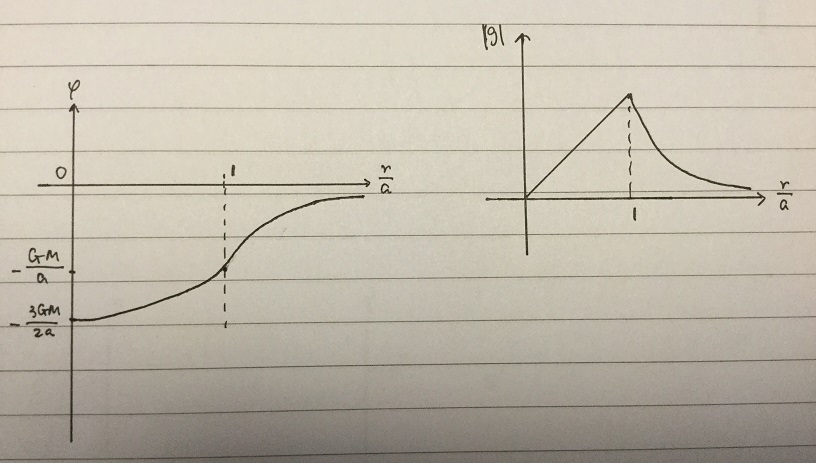
\includegraphics[scale=0.30]{VC11}\\
Alternative solution: use Gauss' law for $\mathbf{g}=g\left(r\right)\mathbf{e}_r$ for $S=$ sphere radius $R$:\\
$\bullet$ $R\geq a$ done before (Newton from Gauss);\\
$\bullet$ $R<a$:
\begin{equation*}
\begin{aligned}
\int_S \mathbf{g}\cdot\mathbf{dS} &= r\pi R^2 g\left(R\right)\\
&= -4\pi GM\left(\frac{R}{a}\right)^3
\end{aligned}
\end{equation*}
So
\begin{equation*}
\begin{aligned}
g\left(R\right) = -\frac{GMR}{a^3}
\end{aligned}
\end{equation*}
for any $R\leq a$.
\end{eg}

To get unique solution of Poisson/Laplace equation, need to impose boundary conditions.\\
Two common kinds of boundary conditions on $\varphi$ at boundary $S=\partial V$ for $\partial$ in volume $V$:\\
$\bullet$ 1) Dirichlet condition (D): specify $\varphi$ on boundary;\\
$\bullet$ 2) Neumann condition (N): specify outward normal derivative $\mathbf{n} \cdot \nabla\varphi$ on boundary. Write $\mathbf{n}\cdot\nabla\varphi = \frac{\partial\varphi}{\partial n}$.\\
(can also impose these on different parts of $\partial V$ or $\alpha \varphi + \beta \frac{\partial \varphi}{\partial n}$ etc.)\\
In applications, boundary conditions generally model physical conditions.\\

\begin{eg}
$\bullet$ Electrostatic potential:\\
(D) $\varphi$ = constant on $S$ for perfectly conducting surface.\\
$\bullet$ Also other equations (of 1B Methods heat/diffusion equation)\\
$T\left(\mathbf{r},t\right)$ the temperature in space and time.\\
(D) $T$ specified on $S$;\\
(N) $\frac{\partial T}{\partial n} = 0$ on S: perfectly insulating boundary.
\end{eg}

\begin{thm} (Uniqueness theorem)\\
Suppose $\varphi\left(\mathbf{r}\right)$ satisfies Poisson equation $\nabla^2\varphi = \rho$ for some $\rho\left(\mathbf{r}\right)$ in a bouded volume $V$, with boundary $S=\partial V$, a closed surface, outward normal $\mathbf{n}$.\\
Then:\\
$\bullet$ 1) if
\begin{equation*}
\begin{aligned}
\varphi\left(\mathbf{r}\right) = f\left(\mathbf{r}\right)
\end{aligned}
\end{equation*}
on $S$ (i.e. D boundary condition), then $\varphi\left(\mathbf{r}\right)$ is unique.\\
$\bullet$ 2) if
\begin{equation*}
\begin{aligned}
\frac{\partial \varphi}{\partial n} = \mathbf{n}\cdot\nabla\varphi = g\left(\mathbf{r}\right)
\end{aligned}
\end{equation*}
on $S$ (i.e. N boundary condition), then $\varphi\left(\mathbf{r}\right)$ is unique up to a constant, i.e. unique up to replacement $\varphi \to \varphi +$ constant.\\
(Note: Laplace equation included as special case $\rho \equiv 0$).
\begin{proof}
Let $\varphi_1\left(\mathbf{r}\right)$ and $\varphi_2\left(\mathbf{r}\right)$ be any two solutions of Poisson equation, with each obeying the boundary conditions (D) or (N) above.\\
Then
\begin{equation*}
\begin{aligned}
\psi\left(\mathbf{r}\right)=\varphi_1\left(\mathbf{r}\right)-\varphi_2\left(\mathbf{r}\right)
\end{aligned}
\end{equation*}
satisfies
\begin{equation*}
\begin{aligned}
\nabla^2\psi = 0
\end{aligned}
\end{equation*}
in $V$, and\\
for (D): $\psi = 0$ on $S$\\
or for (N): $\frac{\partial\psi}{\partial n}=\mathbf{n}\cdot\nabla\varphi = 0$ on $S$.\\
So by divergence theorem(!):
\begin{equation*}
\begin{aligned}
\int_V \nabla\cdot\left(\psi\nabla\psi\right)dV &= \int_S \psi\nabla\psi\cdot\mathbf{dS}\\
&= \int_S \psi \frac{\partial\varphi}{\partial n} dS
\end{aligned}
\end{equation*}
But
\begin{equation*}
\begin{aligned}
\nabla\cdot\left(\psi\nabla\psi\right)&=\nabla\psi\cdot\nabla\psi + \psi\nabla^2\psi\text{(=0 in V)}\\
&= |\nabla\psi|^2
\end{aligned}
\end{equation*}
So
\begin{equation*}
\begin{aligned}
\int_V |\nabla\psi|^2 dV = \int_S \psi \frac{\partial \psi}{\partial n}dS
\end{aligned}
\end{equation*}
But RHS=0 for (D) or (N).\\
(or even if (D) or (N) used on different parts of $S$).\\
Since $|\nabla\psi|^2\geq 0$, $\int_V$ can only vanish if $|\nabla\psi|=0$ i.e. $\nabla\psi = \mathbf{0}$, i.e. $\psi = c$ constant in $V$.\\
So (D): $\psi = 0$ on $S$, so $c=0$, and $\varphi_1 = \varphi_2$ in $V$;\\
or (N): $\frac{\partial\psi}{\partial n} = 0$ on $S$ so any constant $c$ is possible, i.e. $\varphi_1 = \varphi_2 +$ any constant.
\end{proof}
\end{thm}
\begin{rem}
$\bullet$ 1) The theorem says that if a solution exists then its unique, but says nothing about its \emph{existence}.\\
e.g. for (N), if
\begin{equation*}
\begin{aligned}
\nabla^2\varphi = \rho
\end{aligned}
\end{equation*}
in $V$, and
\begin{equation*}
\begin{aligned}
\frac{\partial \varphi}{\partial n} = g
\end{aligned}
\end{equation*}
on $\partial V$, then by divergence theorem,
\begin{equation*}
\begin{aligned}
\int_V \nabla^2\varphi dV = \int_{\partial V} \frac{\partial \varphi}{\partial n}dS
\end{aligned}
\end{equation*}
so
\begin{equation*}
\begin{aligned}
\int_V \rho dV = \int_{\partial V} g dS
\end{aligned}
\end{equation*}
So $\rho$ and $g$ cannot be freely specified independently.\\

$\bullet$ 2) The theorem applies similarly for regions of $\R^n$ for any $n=2,3,4,...$. We need just the definitions of $\grad$, $\vdiv$, and divergence theorem.\\

$\bullet$ 3) The results can be extended to some \emph{un}bounded regions $V$ with suitable asymptotic conditions on $\varphi$ (and then $\psi$ in proof 2 as well, since $\psi = \varphi_1 - \varphi_2$).\\
Consider a sphere of radius $R$ (will take $R\to\infty$):\\
Suppose 
\begin{equation*}
\begin{aligned}
&|\psi\left(\mathbf{r}\right)| = O\left(\frac{1}{R}\right)\\
&|\frac{\partial \psi}{\partial n}| = O\left(\frac{1}{R^2}\right)
\end{aligned}
\end{equation*}
for $|\mathbf{r}| = R$. Then
\begin{equation*}
\begin{aligned}
|\int_S \psi\frac{\partial \psi}{\partial n} dS| &\leq \max_{|\mathbf{r}|\leq R} | \psi \frac{\partial \psi}{\partial n}|\cdot 4\pi R^2\\
&\leq \text{constant   }\cdot \frac{1}{R}\cdot\frac{1}{R^2}\cdot 4\pi R^2\\
&=O\left(\frac{1}{R}\right)\\
&\to 0
\end{aligned}
\end{equation*}
as $R\to\infty$.\\
So uniqueness proof goes through for unbounded region $R\to\infty$.\\
These conditions on $\psi$ and $\frac{\partial \psi}{\partial n}$ are ensured by imposing
\begin{equation*}
\begin{aligned}
|\varphi\left(\mathbf{r}\right)| = O\left(\frac{1}{R}\right) \text{   and   } |\nabla \varphi| = O\left(\frac{1}{R^2}\right)
\end{aligned}
\end{equation*}
so with these asymptotic condition on $\varphi$, the uniqueness theorem extends to all of $\R^3$.\\

$\bullet$ 4) The starting point of proof is a special case of the identity
\begin{equation*}
\begin{aligned}
\nabla \cdot \left(u\nabla v\right) = \nabla u \cdot \nabla v + u \nabla^2 v
\end{aligned}
\end{equation*}
so by divergence theorem
\begin{equation*}
\begin{aligned}
\int_S u\nabla v \mathbf{dS} = \int_S \nabla u \cdot \nabla v dV + \int_V u \nabla^2 v dV
\end{aligned}
\end{equation*}
This is called \emph{Green's first identity}.\\
Swap $u$ and $v$ and subtract the two equations,
\begin{equation*}
\begin{aligned}
\int_S \left(u\nabla v-v\nabla u\right)\cdot \mathbf{dS} = \int_V \left(u\nabla^2 v - v \nabla^2 u\right) dV
\end{aligned}
\end{equation*}
called \emph{Green's second identity}.
\end{rem}

\subsection{Laplace equation and harmonic functions}
Solutions of Laplace equation
\begin{equation*}
\begin{aligned}
\nabla^2 \varphi = 0
\end{aligned}
\end{equation*}
are called \emph{harmonic functions}.

\begin{thm} (Mean value property)\\
Suppose $\varphi\left(\mathbf{r}\right)$ is harmonic in $V$ containing a solid sphere
\begin{equation*}
\begin{aligned}
V_R: |\mathbf{r}-\mathbf{a}| \leq R
\end{aligned}
\end{equation*}
with centre $\mathbf{a}$, with boundary
\begin{equation*}
\begin{aligned}
S_R: |\mathbf{r}-\mathbf{a}| = R
\end{aligned}
\end{equation*}
Then
\begin{equation*}
\begin{aligned}
\varphi\left(\mathbf{a}\right) = \bar{\varphi}\left(R\right)
\end{aligned}
\end{equation*}
where
\begin{equation*}
\begin{aligned}
\bar{\varphi}\left(R\right) = \frac{1}{4\pi R^2}\int_{S_R} \varphi\left(\mathbf{r}\right) dS = \text{   average of  } \varphi \text{   over  } S_R.
\end{aligned}
\end{equation*}
\begin{proof}
Note
\begin{equation*}
\begin{aligned}
\bar{\varphi}\left(R\right) \to \varphi\left(\mathbf{a}\right)
\end{aligned}
\end{equation*}
as $R\to 0$. Take spherical polar coordinates ($u,\theta,\chi$) centred at $\mathbf{a}$.\\
Then on $S_R$ (i.e. $u=R$),
\begin{equation*}
\begin{aligned}
dS = R^2 \sin\theta d\theta d\chi
\end{aligned}
\end{equation*}
So
\begin{equation*}
\begin{aligned}
\bar{\varphi}\left(R\right) = \frac{1}{4\pi R^2}\int_{\chi=0}^{2\pi} \int_{\theta = 0}^\pi \varphi\left(R,\theta,\chi\right) \sin\theta R^2 d\theta d\chi
\end{aligned}
\end{equation*}
So 
\begin{equation*}
\begin{aligned}
\frac{d}{dR} \bar{\varphi}\left(R\right) &= \frac{1}{4\pi} \int_\chi \int_\theta \frac{\partial \varphi}{\partial R}\sin\theta d\theta d\chi\\
&= \frac{1}{4\pi R^2} \int_{S_R} \left(\nabla\varphi \cdot \mathbf{e}_u \right) dS\\
&= \frac{1}{4\pi R^2} \int_{V_R} \nabla^2 \varphi dV\\
&=0
\end{aligned}
\end{equation*}
($\nabla\varphi \cdot \mathbf{e}_u$ takes the first component (at $u=R$), and the second last step is by divergence theorem).\\
Note that $\nabla^2 \varphi = 0$. So $\bar{\varphi}\left(R\right)$ is constant in $R$, so is equal to $\varphi\left(\mathbf{a}\right)$.
\end{proof}
\end{thm}

\begin{defi}
$\varphi\left(\mathbf{r}\right)$ on $V$ has a \emph{local maximum} at $\mathbf{a}\in V$, if for some $\epsilon >0$,
\begin{equation*}
\begin{aligned}
\varphi\left(\mathbf{a}\right) > \varphi\left(\mathbf{r}\right)
\end{aligned}
\end{equation*}
for all $\mathbf{r}\in V$ with $0<|\mathbf{r}-\mathbf{a}|<\epsilon$.\\
(similar for \emph{local minimum}: if $\varphi\left(\mathbf{a}\right)<\varphi\left(\mathbf{r}\right)$ ...)
\end{defi}

\begin{coro}(Maximum of minimum principle)\\
Suppose $\varphi$ is harmonic on $V$. Then $\varphi$ cannot have \emph{any} local maximum or minimum at any interior point of $V$.
\begin{proof}
\emph{if} $\varphi$ has a local maximum at an \emph{interior} point $\mathbf{a}$, there is $\epsilon$ as above so that
\begin{equation*}
\begin{aligned}
\varphi\left(\mathbf{r}\right)<\varphi\left(\mathbf{a}\right)
\end{aligned}
\end{equation*}
for all $|\mathbf{r}-\mathbf{a}|<\epsilon$ and $\mathbf{r}\in V$.\\
By taking $\epsilon$ small enough, we can ensure that the \emph{whole} sphere $\mathbf{r}\in \R^3$ with $|\mathbf{r}-\mathbf{a}|<\epsilon$ lies within $V$ (this is always possible for an \emph{interior} point.)\\
So for any $0<R<\epsilon$, $\varphi\left(\mathbf{r}\right) < \varphi\left(\mathbf{a}\right)$ for $|\mathbf{r}-\mathbf{a}| = R$. So $\bar{\varphi}\left(R\right) < \varphi\left(\mathbf{a}\right)$, contradicting the mean value property.\\
So internal local maximum (similarly minimum) cannot exist.
\end{proof}
\end{coro}

\subsection{Integral solution of Poisson equation}
(Statement and informal derivation)\\
Recall electrostatics: for a point charge $Q$ at $\mathbf{r}_0$, the potential is
\begin{equation*}
\begin{aligned}
\varphi\left(\mathbf{r}\right) = \frac{Q}{4\pi \epsilon_0} \frac{1}{|\mathbf{r}-\mathbf{r}_0|}
\end{aligned}
\end{equation*}
Let's set $\epsilon_0 = 1$.\\
For distribution of charges, density $\rho\left(\mathbf{r}\right)$ all contained in a bounded volume $V'$, the potential satisfies the Poisson equation,
\begin{equation*}
\begin{aligned}
\nabla^2 \varphi = -\frac{\rho}{\epsilon_0} = -\rho
\end{aligned}
\end{equation*}
If we have many point charges $Q_n$ at $\mathbf{r}_\alpha$, then by linearity, the potential is just  the sum:
\begin{equation*}
\begin{aligned}
\varphi\left(\mathbf{r}\right) = \sum_\alpha \frac{1}{4\pi} \frac{Q_\alpha}{|\mathbf{r}-\mathbf{r}_\alpha|}
\end{aligned}
\end{equation*}

Analogously, we can view potential $\varphi$ of density $\rho$ as a sum of contributions
\begin{equation*}
\begin{aligned}
\frac{1}{4\pi}\frac{\rho\left(\mathbf{r}\right)'dV'}{|\mathbf{r}-\mathbf{r}'|}
\end{aligned}
\end{equation*}
from charge elements $\rho\left(\mathbf{r}'\right)dV'$ ranging over $V'$, with $\sum_\alpha$ being replaced by $\int_{V'} dV'$.\\
This suggests that
\begin{equation*}
\begin{aligned}
\varphi\left(\mathbf{r}\right) = \frac{1}{4\pi} \int_V \frac{\rho\left(\mathbf{r}'\right)}{|\mathbf{r}-\mathbf{r}'|}dV'
\end{aligned}
\end{equation*}
is a solution to Poisson equation
\begin{equation*}
\begin{aligned}
\nabla^2\varphi = -\rho
\end{aligned}
\end{equation*}
Here integral is taken with respect to $\mathbf{r}'$ and $\mathbf{r}\in\R^3$ is a parameter in the integral.\\
This is indeed \emph{the} unique solution with boundary condition
\begin{equation*}
\begin{aligned}
&|\varphi\left(\mathbf{r}\right)| = O\left(\frac{1}{|\mathbf{r}|}\right),\\
&|\nabla\varphi\left(\mathbf{r}\right)| = O\left(\frac{1}{|\mathbf{r}|^2}\right)
\end{aligned}
\end{equation*}

\begin{eg}
Using the integral formula, we can calculate again the solution to
\begin{equation*}
\begin{aligned}
\nabla^2\varphi = \left\{
\begin{array}{ll}
-\rho_0 \text{   constant   } & |\mathbf{r}|\leq a\\
0 & |\mathbf{r}|\geq a
\end{array}
\right.
\end{aligned}
\end{equation*}
We have
\begin{equation*}
\begin{aligned}
\varphi\left(\mathbf{r}\right) = \frac{1}{4\pi}\int_{V'} \frac{\rho_0}{|\mathbf{r}-\mathbf{r}'|} dV'
\end{aligned}
\end{equation*}
Here $V'$ is the sphere $|\mathbf{r}'| \leq a$, centred at origin.\\
Introduce spherical polar coordinates $\left(r',\theta,\chi\right)$,\\
(diagram to be inserted -- vc12)\\
with NS pole axis along $\mathbf{r}$, so $\theta$ is the latitude down from $\mathbf{r}$, $\chi$ is the angle around $\mathbf{r}$, and
\begin{equation*}
\begin{aligned}
dV' = r'^2 \sin\theta dr' d\theta d\chi
\end{aligned}
\end{equation*}
By cosine rule for triangle,
\begin{equation*}
\begin{aligned}
|\mathbf{r}-\mathbf{r}'| &= \left(r^2+r'^2 - 2rr' \cos \theta\right) ^\frac{1}{2}
\end{aligned}
\end{equation*}
So
\begin{equation*}
\begin{aligned}
\varphi\left(\mathbf{r}\right) &= \frac{1}{4\pi} \int_0^a dr' \int_0^\pi d\theta \int_0^{2\pi} d\chi \frac{\rho_0 r'^2\sin\theta}{\sqrt{r^2+r'^2-2rr'\cos\theta}}\\
&=\frac{\rho_0}{2} \int_0^a dr' r'^2 \frac{1}{rr'}\left[\sqrt{r^2+r'^2 - 2rr'\cos\theta}\right]_{\theta=0}^{\theta=\pi}
\end{aligned}
\end{equation*}
While 
\begin{equation*}
\begin{aligned}
\left[\sqrt{r'^2+r^2-2rr'\cos\theta}\right]_0^\pi = \left[|\mathbf{r}-\mathbf{r'}|\right]_{\theta=0}^{\theta=\pi}
\end{aligned}
\end{equation*}
when $\theta =\pi$: $\mathbf{r}$, $\mathbf{r'}$ are antiparallel. So $|\mathbf{r}-\mathbf{r}'| = r+r'$;\\
when $\theta = 0:$ $\mathbf{r}$, $\mathbf{r'}$ are parallel. So $|\mathbf{r}-\mathbf{r'}| = |r-r'|$.\\
Then
\begin{equation*}
\begin{aligned}
\left(r+r'\right) - |r-r'| = \left\{
\begin{array}{ll}
2r' & r>r'\\
2r & r<r'
\end{array}
\right.
\end{aligned}
\end{equation*}
So
\begin{equation*}
\begin{aligned}
\varphi\left(\mathbf{r}\right) = \left\{
\begin{array}{ll}
\rho_0 \int_0^a dr' \frac{r'^2}{r} & r>a\\
\rho_0 \int_0^r dr' \frac{r'^2}{r} + \rho_0\int_r^a dr' r' & r\leq a
\end{array}
\right.
\end{aligned}
\end{equation*}
In the first case $r>r'$ as $r'<a$, in the second case $r'$ varies from $0\to a$ so separable: $r':0\to r(r'<r)$ and $r\to a(r'>r)$. So
\begin{equation*}
\begin{aligned}
\varphi\left(\mathbf{r}\right) = \left\{
\begin{array}{ll}
\rho_0 \frac{1}{3}a^3 \frac{1}{r} & r>a\\
\rho_0 \left(-\frac{1}{b}r^2 + \frac{1}{2}a^2\right) & r\leq a
\end{array}
\right.
\end{aligned}
\end{equation*}
\emph{as before}.

\subsection{Point sources and delta functions (non-examinable)}
For
\begin{equation*}
\begin{aligned}
\varphi\left(\mathbf{r}\right) = \frac{1}{4\pi} \int_{V'} \frac{\rho\left(\mathbf{r}'\right)}{|\mathbf{r}-\mathbf{r'}|} dV'
\end{aligned}
\end{equation*}
We have
\begin{equation}\label{eq:10}
\begin{aligned}
\nabla^2 \varphi = \frac{1}{4\pi} \int_{V'} \rho \left(\mathbf{r}'\right) \nabla^2 \left(\frac{1}{|\mathbf{r}-\mathbf{r}'|}\right) dV'
\end{aligned}
\end{equation}
Write $\mathbf{r}' = \mathbf{a}$ consider
\begin{equation*}
\begin{aligned}
\psi = \frac{1}{4\pi}\frac{1}{|\mathbf{r}-\mathbf{a}}
\end{aligned}
\end{equation*}
then calculate
\begin{equation*}
\begin{aligned}
&\nabla\psi = -\frac{1}{4\pi} \frac{\mathbf{r}-\mathbf{a}}{|\mathbf{r}-\mathbf{a}|^3},\\
&\nabla^2 \psi = 0(!)
\end{aligned}
\end{equation*}
for all $\mathbf{r}\neq \mathbf{a}$.\\
Note these are all singular at $\mathbf{a}=\mathbf{a}$ and \emph{ok} for all $\mathbf{r}\neq \mathbf{a}$.\\

\begin{equation*}
\begin{aligned}
\int_S \nabla\psi \cdot \mathbf{dS} = -1
\end{aligned}
\end{equation*}
(e.g. by using $|\mathbf{r}-\mathbf{a}|$ = radial coordinates $u$, $\left(\mathbf{r}-\mathbf{a}\right) = u \mathbf{e}_u$ etc) for $S$ surface of any sphere $V$, centre $\mathbf{a}$.\\
So divergence theorem would require (!):
\begin{equation*}
\begin{aligned}
\int_V \nabla^2 \psi dV = -1
\end{aligned}
\end{equation*}
$\nabla^2 \psi$ is zero for all $\mathbf{r}\neq \mathbf{a}$.\\
This holds if we take
\begin{equation*}
\begin{aligned}
\nabla^2 \left(\frac{1}{4\pi} \frac{1}{|\mathbf{r}-\mathbf{a}|}\right) = -\delta \left(\mathbf{r}-\mathbf{a}\right)
\end{aligned}
\end{equation*}
RHS is a 3-D delta function -- a generalised function satisfying
\begin{equation*}
\begin{aligned}
\int_V f\left(\mathbf{r}\right) \delta \left(\mathbf{r}-\mathbf{a}\right) dV = f\left(\mathbf{a}\right)
\end{aligned}
\end{equation*}
for any $V$ containing $\mathbf{a}$.\\
Then (\ref{eq:10}) gives
\begin{equation*}
\begin{aligned}
\nabla^2 \varphi = -\rho \left(\mathbf{r}\right) 
\end{aligned}
\end{equation*}
as wanted.\\
For point source $Q$ at $\mathbf{a}$, the potential
\begin{equation*}
\begin{aligned}
&\varphi\left(\mathbf{r}\right) = \frac{Q}{4\pi} \frac{1}{|\mathbf{r}-\mathbf{a}|}\\
&\nabla^2 \varphi = -Q\delta \left(\mathbf{r}-\mathbf{a}\right)=-\text{   charge density of point source  } Q \text{  at  } \mathbf{r} = \mathbf{a}
\end{aligned}
\end{equation*}
This is zero except $\mathbf{r}=\mathbf{a}$, infinite at $\mathbf{r}=\mathbf{a}$, but any $\int_V$ about $\mathbf{a}$ gives $Q$.
\end{eg}

\newpage
\section{Maxwell's equations}
Laws of electromagnetism(full dynamic case).\\
Let\\
$\mathbf{E}\left(\mathbf{r},t\right)$ be the electric field,\\
$\mathbf{B}\left(\mathbf{r},t\right)$ be the magnetic field,\\
$\rho\left(\mathbf{r},t\right)4$ be charge density,\\
$\mathbf{j}\left(\mathbf{r},t\right)$ be current density.\\
Then
\begin{equation*}
\begin{aligned}
&\nabla \cdot \mathbf{E} = V_{\epsilon_0} & (1)\\
&\nabla\times\mathbf{E} + \frac{\partial \mathbf{B}}{\partial t} = 0 & (2)\\
&\nabla\cdot \mathbf{B} = 0 & (3)\\
& \nabla\times\mathbf{B}-\mu_0 \epsilon_0 \frac{\partial \mathbf{E}}{\partial t} = \mu_0 \mathbf{j} & (4)
\end{aligned}
\end{equation*}
($\epsilon_0$, $\mu_0$ are respectively the permittivity and permeability of free space -- constants).\\

\begin{thm} (Lorentz force law)\\
The force on a point charge $q$ at $\mathbf{r}\left(t\right)$ due to $\mathbf{E}$ and $\mathbf{B}$ fields is
\begin{equation*}
\begin{aligned}
\mathbf{F} = q\left(\mathbf{E}+\dot{\mathbf{r}}\times\mathbf{B}\right)
\end{aligned}
\end{equation*}
\end{thm}

\subsection{Conservation of electric charge from Maxwell equation}
Take the div of the fourth equation and use the first one,
\begin{equation*}
\begin{aligned}
-\mu_0 \epsilon_0 \frac{\partial}{\partial t}\left(\frac{\rho}{\epsilon_0}\right) = \mu_0 \nabla \cdot \mathbf{j}
\end{aligned}
\end{equation*}
So
\begin{equation*}
\begin{aligned}
\frac{\partial \rho}{\partial t} + \nabla \cdot \mathbf{j} = 0
\end{aligned}
\end{equation*}
i.e. the conservation and continuity of equation for $\rho, \mathbf{j}$.

Integral forms:\\
For (1) and (3) use divergence theorem, and get respectively:
\begin{equation*}
\begin{aligned}
\int_S \mathbf{e}\cdot \mathbf{dS} = \frac{Q}{\epsilon_0}\\
\int_S \mathbf{B}\cdot \mathbf{dS} = 0
\end{aligned}
\end{equation*}
Here $S$ is any closed surface, enclosing charge. For (2) and (4), use Stokes' Theorem. For (2):
\begin{equation*}
\begin{aligned}
\int_C \mathbf{E}\cdot \mathbf{dr} = -\frac{d}{dt}\int_S \mathbf{B}\cdot \mathbf{dS}
\end{aligned}
\end{equation*}
$S$ is any surface with closed curve boundary $C$.\\
For (4):
\begin{equation*}
\begin{aligned}
\int_C \mathbf{B}\cdot\mathbf{dr} = \mu_0 \int \mathbf{j}\cdot \mathbf{dS} + \mu_0 \epsilon_0 \frac{d}{dt}\int \mathbf{E}\cdot \mathbf{dS}
\end{aligned}
\end{equation*}

Fully static case: $\rho$, $\mathbf{j}$, $\mathbf{E}$, $\mathbf{B}$ are all time independent. Then $\mathbf{E}$ and $\mathbf{B}$ decouple in the equations (not related in a single equation).\\
$\bullet$ Electrostatics:
\begin{equation*}
\begin{aligned}
&\nabla\cdot\mathbf{E} = \frac{\rho}{\epsilon_0}\\
&\nabla\times\mathbf{E} = 0\\
&\mathbf{E} = -\nabla\varphi\\
&\nabla^2 \varphi = -\frac{\rho}{\epsilon_0}
\end{aligned}
\end{equation*}
$\varphi$ is the electrostatic potential, satisfies scalar Poisson equation.\\

$\bullet$ Magnets statics:
\begin{equation*}
\begin{aligned}
&\nabla\cdot \mathbf{B} = 0 \implies B = \nabla\times\mathbf{A}\\
&\nabla\times\mathbf{B} = \mu_0 \mathbf{j}
\end{aligned}
\end{equation*}
Here $\mathbf{A}$ is a vector potential (true in field case too). The freedom in choice of $\mathbf{A}$ is 
\begin{equation*}
\begin{aligned}
\mathbf{A} \to \mathbf{A} + \nabla \chi
\end{aligned}
\end{equation*}
for any $\chi$ (called \emph{gauge freedom}).\\

We can choose $\chi$ to make
\begin{equation*}
\begin{aligned}
\nabla\cdot\mathbf{A} = 0 \text{  } \nabla^2\chi \cong -\text{previous  } \div \mathbf{A}
\end{aligned}
\end{equation*}
Then
\begin{equation*}
\begin{aligned}
\nabla\times\mathbf{B} = \nabla\times\left(\nabla\times\mathbf{A}\text{ =0 }\right) = \nabla\left(\nabla\cdot\mathbf{A}\right)-\nabla^2 \mathbf{A}
\end{aligned}
\end{equation*}
So
\begin{equation*}
\begin{aligned}
\nabla^2 \mathbf{A} = -\mu_0 \mathbf{j}
\end{aligned}
\end{equation*}
the \emph{vector} Poisson equation for $\mathbf{A}$.

\subsection{Electromagnetic waves}
Consider Maxwell equation in empty space, i.e.
\begin{equation*}
\begin{aligned}
\rho = 0, \mathbf{j} = 0
\end{aligned}
\end{equation*}
Then as shown previously
\begin{equation*}
\begin{aligned}
\nabla^2 \mathbf{E} &= \nabla\left(\nabla\cdot\mathbf{E}  \text{ =0 }\right)-\nabla\times\left(\nabla\times\mathbf{E}\right)\\
&= \nabla\times\frac{\partial \mathbf{B}}{\partial t}\\
&= \frac{\partial}{\partial t}\left(\mu_0 \epsilon_0 \frac{\partial \mathbf{E}}{\partial t}\right) \\
&= \mu_0 \epsilon_0 \frac{\partial^2 \mathbf{E}}{\partial t^2}
\end{aligned}
\end{equation*}
i.e.,
\begin{equation*}
\begin{aligned}
\left(\nabla^2 - \frac{1}{c^2}\frac{\partial^2}{\partial t^2}\right) \mathbf{E} = \mathbf{0}
\end{aligned}
\end{equation*}
and get same for $\mathbf{B}$, where $c^2 = \frac{1}{\epsilon_0 \mu_0}$.\\
i.e. compounds of $\mathbf{E}$ and $\mathbf{B}$ satisfy wave equation in 3 dimensions with speed of propagation
\begin{equation*}
\begin{aligned}
c=\frac{1}{\sqrt{\epsilon_0 \mu_0}}
\end{aligned}
\end{equation*}

Recall 1D wave equation:
\begin{equation*}
\begin{aligned}
\left(\frac{\partial^2}{\partial x^2} - \frac{1}{c^2}\frac{\partial^2}{\partial t^2}\right) f\left(x,t\right) = 0
\end{aligned}
\end{equation*}
has solutions
\begin{equation*}
\begin{aligned}
f\left(x,t\right) = f\left(x\pm ct\right)
\end{aligned}
\end{equation*}
For $f\left(x-ct\right),f\left(x+ct\right)$: right/left moving wave, shape $f\left(x\right)$.\\
So Maxwell's equations predict the existence of electromagnetic waves moving at speed
\begin{equation*}
\begin{aligned}
c=\frac{1}{\sqrt{\epsilon_0 \mu_0}}=2.998*10^8 m/sec
\end{aligned}
\end{equation*}
from measured value of $\epsilon_0$, $\mu_0$. i.e. we get expected value of speed of light!\\
Light identified as waves of electromagnetism.

\newpage
\section{Tensors}
\subsection{Introduction}
A generalisation of idea of vectors as \emph{geometrical objects}.\\
Consider a vector $\mathbf{v}$ in space (e.g. velocity of a particle).
It is described by 3 real numbers (components) only after we have chosen a basis ( or Cartesian coordinates).\\
The components depend on the \emph{choice} of basis.\\
But $\mathbf{v}$ (velocity) has physical significance (existence independent of choice of any basis, i.e. it is a geometrical object).\\
To get a description independent of any \emph{particular choice} of basis, we can give its components for all possible choices of orthonormal bases.\\
Consider right-handed orthonormal bases
\begin{equation*}
\begin{aligned}
B=\left\{\mathbf{e}_i\right\},B' = \left\{\mathbf{e}_i'\right\}
\end{aligned}
\end{equation*}
in 3D space, any such bases related by \emph{rotation} $R$
\begin{equation*}
\begin{aligned}
\mathbf{e}_i' = R_{ip} \mathbf{e}_p
\end{aligned}
\end{equation*}
For any vector
\begin{equation*}
\begin{aligned}
\mathbf{v}=v_i \mathbf{e}_i = v_i' \mathbf{e}_i'
\end{aligned}
\end{equation*}
components are related by
\begin{equation*}
\begin{aligned}
v_i' = R_{ip}v_p
\end{aligned}
\end{equation*}
Recall: rotation matrix $R$ has
\begin{equation*}
\begin{aligned}
RR^T = R^TR = I
\end{aligned}
\end{equation*}
i.e.
\begin{equation*}
\begin{aligned}
R_{ip}R_{jp} = R_{qi} R_{qj} = \delta_{ij}
\end{aligned}
\end{equation*}
So 
\begin{equation}\label{eq:11}
\begin{aligned}
R_{ip} R_{jq}\delta_{pq} = \delta_{ij}
\end{aligned}
\end{equation}
We have $\det R = 1$, so
\begin{equation}\label{eq:12}
\begin{aligned}
\epsilon_{pqr} R_{ip} R_{jq} r_{kr} = \epsilon_{ijk} \det R = \epsilon_{ijk}
\end{aligned}
\end{equation}
So a vector $\mathbf{v}$ is a triple of numbers $\left(v_1,v_2,v_3\right)$ for each orthonormal basis $B=\left\{\mathbf{e}_i\right\}$ such that if $B'$ is related to $B$ by rotation $R$ (as above), the corresponding triples are related by
\begin{equation*}
\begin{aligned}
v'_i = R_{ip} v_p
\end{aligned}
\end{equation*}
called the \emph{vector transformation rule}.

\begin{defi}
A (Cartesian) tensor of rank $n$ has components $T_{ij...k}$ ($n$ indices) with respect to each orthonormal basis $B=\left\{\mathbf{e}_i\right\}$ satisfying the \emph{tensor transformation law}:
\begin{equation*}
\begin{aligned}
T'_{ij...k} = R_{ip} R_{jq} ... R_{kr} T_{pq...r}
\end{aligned}
\end{equation*}
when bases $B$ and $B'$ are related by rotation $R$.
\end{defi}

\begin{eg}
Tensor of rank 0: no indices, $T=T'$ -  a scalar.\\
Tensor of rank 1: $T'_i = R_{ip} T_p$ - a vector.\\
Tensor of rank 2: $T'_{ij} = R_{ip} R_{jq} T_{pq}$ - components form a matrix.\\
If $\mathbf{u}$, $\mathbf{v}$, ... $\mathbf{w}$ are $n$ vectors, then 
\begin{equation*}
\begin{aligned}
T_{ij...k} = u_i v_j ... w_k
\end{aligned}
\end{equation*}
is a tensor of rank $n$ called \emph{outer product} or \emph{tensor product} of vectors.
\end{eg}

Note that (\ref{eq:11}) and (\ref{eq:12}) say exactly that $\delta_{ij}$ and $\epsilon_{ijk}$ are tensors of ranks 2 and 3 with \emph{special property} that their components are the same with respect to any basis or coordinate system - called \emph{isotropic} or \emph{invariant tensors}.

\subsection{Rank 2 tensors, linear map, matrices}
Linear map on vectors represented as a matrix on components, given a choice of basis.\\
e.g. $B$ or $B'$:\\
\begin{equation}\label{eq:13}
\begin{aligned}
v_i = M_{ij} u_j \text{  or  } v'_i = M'_{ij} u'_j
\end{aligned}
\end{equation}
Matrix depends on the choice of basis.\\
If 
\begin{equation*}
\begin{aligned}
\mathbf{e}'_i = R_{ij} \mathbf{e}_j
\end{aligned}
\end{equation*}
where $R$ is the rotation matrix, then
\begin{equation*}
\begin{aligned}
M' = RMR^{-1}
\end{aligned}
\end{equation*}
But $R$ is a rotation matrix, so orthogonal. So
\begin{equation*}
\begin{aligned}
M'_{ij} = R_{ip} M _{pq} \left(R^{-1}\right)_{qj} = R_{ip} M_{pq} R_{jq}
\end{aligned}
\end{equation*}
i.e. $M$ satisfies rank 2 tensor transformation law.
(can also see this from (\ref{eq:13}) by substituting vectors transformation laws:
\begin{equation*}
\begin{aligned}
v'_i = R_{ij}v_j, v_j = R_{ij} v'_i
\end{aligned}
\end{equation*}

\begin{eg} (Conductivity tensor)\\
In many substances, applied electric field $\mathbf{E}$ induces a current density $\mathbf{j}$ via a linear relation (Ohm's Law):
\begin{equation*}
\begin{aligned}
j_i = \sigma_{ik} E_k
\end{aligned}
\end{equation*}
so by the above $\sigma$ is a tensor -- called conductivity tensor.\\
In general, substances may conduct differently in different directions and $\mathbf{j}$ not parallel to $\mathbf{E}$.\\
For isotropic substance, $\sigma_{ik} = \sigma \delta_{ik}$, so $\mathbf{j} = \sigma \mathbf{E}$ and they are parallel.
\end{eg}

\subsection{Tensor algebra}
\subsubsection{Addition and scalar multiplication}
If $S,T$ are tensors of some rank $n$, then:\\
$\bullet$ $\left(S+T\right)$ \emph{defined} by (in any basis):
\begin{equation*}
\begin{aligned}
\left(S+T\right){ij...k} = S_{ij...k} + T_{ij...k}
\end{aligned}
\end{equation*}
$\bullet$ $\alpha T$ for scalar and defined by
\begin{equation*}
\begin{aligned}
\left(\alpha T\right)_{ij...k} = \alpha T_{ij...k}
\end{aligned}
\end{equation*}
are also \emph{tensors} of rank $n$.\\
(easy e.g. for rank 2:\\
\begin{equation*}
\begin{aligned}
\left(S+T\right)'_{ij} &= S'_{ij} + T'_{ij}\\
&= R_{ip} R_{jq} S_{pq} + R){ip} R_{jq} T_{pq}\\
&= R_{ip} R_{jq} \left(S_{pq} + T_{pq}\right)\\
&= R_{ip} R_{jq} \left(S+T\right)_{pq}
\end{aligned}
\end{equation*}

\subsubsection{Tensor products}
If $S,T$ are tensors of ranks $m,n$ respectively, then the tensor product $S\otimes T$ has rank $m+n$, and is defined by
\begin{equation*}
\begin{aligned}
\left(S\otimes T\right)_{ij...k pq...r} = S_{ij...k} T_{pq...r}
\end{aligned}
\end{equation*}
clearly satisfies correct transformation rule (for $m+n$ suffixes).\\
The definition of $S\otimes T\otimes U\otimes...$ is similar.\\
$\otimes$ is associative, but \emph{not} commutative.\\
E.g. vectors $\mathbf{u}$, $\mathbf{v}$,
\begin{equation*}
\begin{aligned}
T=u\otimes v
\end{aligned}
\end{equation*}
has components $T_{ij} = u_i v_j$, but
\begin{equation*}
\begin{aligned}
S=v\otimes u
\end{aligned}
\end{equation*}
has components $S_{ij} = v_i u_j$.\\

\subsubsection{Contractions}
For rank $n$ tensor $T_{ijp...q}$, introduce $S_{p...q}$ with $\left(n-2\right)$ indices defined by
\begin{equation*}
\begin{aligned}
S_{p...q} = \delta_{ij} T_{ijp...q} = T_{iip...q}
\end{aligned}
\end{equation*}
i.e. \emph{contracting} the two indices $i$ and $j$.\\
Then $S$ is a \emph{tensor} of rank $\left(n-2\right)$.\\
To prove this, see
\begin{equation*}
\begin{aligned}
S'_{p...q} &= \delta_{ij} T'_{ijp...q}\\
&= \delta_{ij} R_{ia} R_{jb} R_{pc} ... R_{qd} T_{abc...d}\\
&= \delta_{ab} R_{pc} ... R_{qd} T_{abc...d}\\
&= R_{pc} ... R_{qd} S_{c...d}
\end{aligned}
\end{equation*}
which is the correct transformation law for $n-2$ indices.\\

\begin{eg}
For rank 2 tensors: scalar $T_{ii}$ = trace of $3\times 3$ matrix $T_{ij}$.\\
in matrix notation:
\begin{equation*}
\begin{aligned}
T'_{ii} = \tr\left(T'\right) = \tr\left(RTR^T\right) = \tr\left(T\right) = T_{ii}.
\end{aligned}
\end{equation*}
\end{eg}

\subsection{Symmetric and antisymmetric tensors}
If 
\begin{equation*}
\begin{aligned}
T_{...i...j...} = \left\{
\begin{array}{ll}
+T_{...j...i...} & T \text{  symmetric in index i,j}\\
-T_{...j...i...} & T \text{  antisymmetric in index i,j}
\end{array}
\right.
\end{aligned}
\end{equation*}
(If this holds in one coordinate system, then it holds in all of the systems).\\
$T$ is \emph{totally} symmetric/antisymmetric if it is symmetric/antisymmetric in all pairs of indices.\\

\begin{eg}
$\delta_{ij}$ is totally symmetric rank 2 tensor.\\
$\epsilon_{ijk}$ is totally antisymmetric rank 3 tensor.
\end{eg}

For any $n$, there are totally symmetric tensors of rank $n$. e.g.: Let $u$ be a vector, $T_{ij...k} = u_i u_j ... u_k$.\\
In 3D:\\
any totally antisymmetric rank 3 tensor $T$ has the form
\begin{equation*}
\begin{aligned}
T_{ijk} = \lambda \epsilon_{ijk}
\end{aligned}
\end{equation*}
since, if $T_{123} = \lambda$, then all the other components are fixed to be $\pm \lambda$ or 0 due to antisymmetry.\\
Any totally anti-symmetric tensor $T$ of rank greater than 3 must be trivial, i.e. $T=0$. This is because for any choice of more than 3 indices $ij...k \in \left\{1,2,3\right\}$ in $T_{ij...k}$, at least two of them must be the same.

\subsection{Tensors as multi-linear maps, quotient rule}
Multi-linear map $T$ from $n$ vectors $\mathbf{a},\mathbf{b},...\mathbf{c}$ to $\R$ is the map $T\left(\mathbf{a},\mathbf{b},...,\mathbf{c}\right)$ that is linear in each vector separately.\\
So in a basis $B=\left\{\mathbf{e}_i\right\}$, $\mathbf{a} = a_i \mathbf{e}_i$ etc.\\
Linearity gives
\begin{equation*}
\begin{aligned}
T\left(\mathbf{a}, \mathbf{b},...,\mathbf{c}\right) = T_{ij...k} a_i b_j ... c_k
\end{aligned}
\end{equation*}
where the coefficients
\begin{equation*}
\begin{aligned}
T_{ij...k}  = T\left(\mathbf{e}_i, \mathbf{e}_j,...,\mathbf{e}_k\right)
\end{aligned}
\end{equation*}
For any other basis $B'=\left\{\mathbf{e}'_i\right\}$ related by rotation $R$,
\begin{equation*}
\begin{aligned}
T'_{ij...k} &= T\left(\mathbf{e}'_i, \mathbf{e}'_j, ..., \mathbf{e}'_k\right)\\
&= T\left(R_{ip} \mathbf{e}_p, R_{jq} \mathbf{e}_q, ..., R_{kr} \mathbf{e}_r\right)\\
&= R_{ip} R_{jq} ... R_{kr} T_{pq...r}
\end{aligned}
\end{equation*}
So $T_{ij...k}$ \emph{is} a tensor of rank $n$.

Conversely, given a tensor $T$ of rank $n$, define $T\left(\mathbf{a},\mathbf{b},...,\mathbf{c}\right)$ to be
\begin{equation*}
\begin{aligned}
T_{ij...k} a_i b_j ... c_k
\end{aligned}
\end{equation*}
for components in some basis - \emph{independent} of choice of basis (as $T$ is a tensor and have contractions) so defines a multi-linear map on \emph{vectors}.\\
Thus there is a 1-1 correspondence between rank $n$ tensors and multi-linear maps from $n$ vector to $\R$.

\subsection{Quotient rule}
We know that if $T_{i...jp...q}$ ($n$ indices in $i...j$ and $m$ indices in $p...q$) is a tensor of rank $m+n$ and $u_{p...q}$ is any tensor of rank $m$, then contraction
\begin{equation*}
\begin{aligned}
v_{i...j} = T_{i...jp...q} u_{p...q}
\end{aligned}
\end{equation*}
is a tensor of rank $n$.\\
The converse is called \emph{quotient rule}:
Suppose $T_{i...jp...q}$ is any array of numbers (given for each basis) such that for any tensor $u_{p...q}$,
\begin{equation*}
\begin{aligned}
v_{i...j} = T_{i...jp...q} u_{p...q}
\end{aligned}
\end{equation*}
is a \emph{tensor} of rank $n$, then $T_{i...jp...q}$ is also a tensor (rank $m+n$).
\begin{proof}
take
\begin{equation*}
\begin{aligned}
u_{p...q} = c_{p}...d_q
\end{aligned}
\end{equation*}
for $m$ vectors $\mathbf{c},...,\mathbf{d}$. Then some $v_{i...j}$ is a \emph{tensor}.\\
We have: for any $n$ vectors $\mathbf{a},...,\mathbf{b}$,
\begin{equation*}
\begin{aligned}
v_{i...j} a_i... b_j = T_{i...jp...q} a_i...b_j c_p...d_q
\end{aligned}
\end{equation*}
is \emph{scalar}, so define a multi-linear map on $m+n$ vectors so coefficients $T_{i...q}$ must be a tensor (of rank $m+n$).
\end{proof}

\subsection{Tensor calculus}
A tensor \emph{field} is a tensor $T_{ij...k} \left(\mathbf{x}\right)$ at each point.\\
It is smooth if each component function is smooth (in \emph{any} coordinate system).\\
Then the \emph{derivative}
\begin{equation*}
\begin{aligned}
\frac{\partial}{\partial x_p}...\frac{\partial}{\partial x_q} T_{ij...k}
\end{aligned}
\end{equation*}
($m$ of the partial derivatives) is a new \emph{tensor} of rank $\left(m+n\right)$.\\
Correct transformation law on new indices follows from Chain rule: if
\begin{equation*}
\begin{aligned}
x'_p = R_{pq}x_q
\end{aligned}
\end{equation*}
($R$ rotation, constant) then
\begin{equation*}
\begin{aligned}
\frac{\partial}{\partial x'_p} = R_{pq} \frac{\partial}{\partial x_q}
\end{aligned}
\end{equation*}
so e.g. rank $T$ and one derivative
\begin{equation*}
\begin{aligned}
\frac{\partial T'_i}{\partial x'_p} = R_{pq} \frac{\partial}{\partial x_q} \left(R_{ij}T_j\right) = R_{pq}R_{ij} \left(\frac{\partial T_j}{\partial x_c}\right)
\end{aligned}
\end{equation*}

\emph{Integrals}: of a tensor field e.g.
\begin{equation*}
\begin{aligned}
\int_V T_{ij...k} dV
\end{aligned}
\end{equation*}
is defined by integrals of component functions. The transformation rule for the result holds (so it's still a tensor). e.g. integrals are limits of sums.\\

The divergence theorem can be generalised from vectors to tensors:

\begin{thm}
Let $V$ be a volume bounded by smooth closed surface $S=\partial V$, outward unit normal $\mathbf{n}$, and let $T_{ij...kl}$ be a smooth tensor field. Then
\begin{equation}\label{eq:14}
\begin{aligned}
\int_S T_{ij...kl} n_l dS = \int_V \frac{\partial}{\partial x_l} \left(T_{ij...kl}\right) dV
\end{aligned}
\end{equation}
\begin{proof}
apply vector divergence theorem to vector field $\mathbf{f}$ defined by
\begin{equation*}
\begin{aligned}
v_l = a_i b_j ... c_k T_{ij...kl}
\end{aligned}
\end{equation*}
where $\mathbf{a}$, $\mathbf{b}$, ... $\mathbf{c}$ are any constant vectors. Then
\begin{equation*}
\begin{aligned}
&\nabla\cdot\mathbf{v} = \frac{\partial v_l}{\partial x_l} = a_i b_j ... c_k \frac{\partial}{\partial x_l} T_{ij...kl}\\
&\mathbf{n}\cdot\mathbf{v} = a_i b_j ... c_k T_{ij...kl} n_l
\end{aligned}
\end{equation*}
\end{proof}
so we get (\ref{eq:14}) contracted with $a_i b_j ... c_k$ on both sides.\\
Setting $\mathbf{a}$, $\mathbf{b}$, ..., $\mathbf{c}$ to all choice of basis vectors gives (\ref{eq:14}).
\end{thm}

\subsection{Tensors of rank 2}
\emph{Decomposition}: any $T_{ij}$ can be written as sum of symmetric and anti-symmetric parts:
\begin{equation*}
\begin{aligned}
T_{ij} = S_{ij} + A_{ij}
\end{aligned}
\end{equation*}
where
\begin{equation*}
\begin{aligned}
S_{ij} = \frac{T_{ij} + T_{ji}}{2},\\
A_{ij} = \frac{T_{ij} - T_{ji}}{2}
\end{aligned}
\end{equation*}
Then further reduce symmetric part:
\begin{equation*}
\begin{aligned}
S_{ij} = P_{ij} + \frac{1}{3}\delta_{ij} Q
\end{aligned}
\end{equation*}
with $P_{ij}$ traceless (i.e. $P_{ii} = 0$) and $Q=S_{ii} = T_{ii}$, since $A_{ii} = 0$.\\
If $T$ is a tensor then $A,S,P,Q$ are all tensors too.\\
\begin{equation*}
\begin{aligned}
\text{Tensor} & \text{          } & \text{no. of independent components}\\
T & & 9\\
A & & 3\\
S & & 6\\
P & & 5\\
Q & & 1
\end{aligned}
\end{equation*}
For anti-symmetric: any anti-symmetric $3\times 3$ matrix $A$ can be written
\begin{equation*}
\begin{aligned}
\left(A_{ij}\right) = \left[
\begin{matrix}
0 & B_3 & -B_2 \\
-B_3 & 0 & B_1 \\
B_2 & -B_1 & 0 \\
\end{matrix}\right]
\end{aligned}
\end{equation*}
Then 
\begin{equation*}
\begin{aligned}
A_{ij} = \epsilon_{ijk} B_k
\end{aligned}
\end{equation*}
because (what?)\\
$\epsilon-\delta$ identity:
\begin{equation*}
\begin{aligned}
B_k = \frac{1}{2} \epsilon_{ijk} A_{ij} \iff A_{ij} = \epsilon_{ijk} B_k
\end{aligned}
\end{equation*}
Note also
\begin{equation*}
\begin{aligned}
B_k = \frac{1}{2}\epsilon_{ijk} T_{ij}
\end{aligned}
\end{equation*}
as $\epsilon_{ijk} \delta_{ij} = 0$.\\
Summary:
\begin{equation*}
\begin{aligned}
T_{ij} = P_{ij} + \epsilon_{ijk} B_k + \frac{1}{3}\delta_{ij} Q
\end{aligned}
\end{equation*}
where
\begin{equation*}
\begin{aligned}
&B_k = \frac{1}{2}\epsilon_{ijk} T_{ij}\\
&Q = T_{kk}\\
&P_{ij} = \frac{T_{ij} + T_{ji}}{2} - \frac{1}{3} \delta_{ij} T_{kk}
\end{aligned}
\end{equation*}

\begin{eg}
If $F_i\left(\mathbf{r}\right)$ is a vector field, then its derivative $T_{ij} = \frac{\partial F_i}{\partial x_j}$ is rank 2 tensor with
\begin{equation*}
\begin{aligned}
&P_{ij} = \frac{1}{2}\left(\frac{\partial F_i}{\partial x_j} + \frac{\partial F_j}{\partial x_i}\right) - \frac{1}{3}\delta_{ij} \left(\nabla\cdot\mathbf{F}\right)\\
&B_k = \frac{1}{2}\epsilon_{ijk} \frac{\partial F_i}{\partial x_j} = -\frac{1}{2} \left(\nabla\times\mathbf{F}\right)_k\\
&Q = \frac{\partial F_k}{\partial x_k} = \nabla\cdot\mathbf{F}.
\end{aligned}
\end{equation*}
\end{eg}

\subsection{The inertia tensor}
Consider masses $m_\alpha$, position $\mathbf{r}_\alpha$, all rotating with angular velocity $\mathbf{\omega}$ about $\mathbf{0}$.\\
So velocities $\mathbf{v}_\alpha = \mathbf{\omega} \times \mathbf{r}_\alpha$.\\
Total angular momentum about $\mathbf{0}$ is
\begin{equation*}
\begin{aligned}
\mathbf{L} = \sum_\alpha \mathbf{r}_\alpha \times m_\alpha \mathbf{v}_\alpha = \sum m_\alpha \mathbf{r}_\alpha \times \left(\mathbf{\omega} \times \mathbf{r}_\alpha\right)
\end{aligned}
\end{equation*}
In components $L_i = I_{ij} \omega_j$, where
\begin{equation*}
\begin{aligned}
I_{ij} = \sum_\alpha m_\alpha \left(\left(\mathbf{r}_\alpha\right)_k \left(\mathbf{r}_\alpha\right)_k \delta_{ij} - \left(\mathbf{r}_\alpha\right)_i \left(\mathbf{r}_\alpha\right)_j\right)
\end{aligned}
\end{equation*}
is the \emph{inertia tensor} about $\mathbf{0}$.

\end{document}